The AGWB is not independent of the observed frequency of the GW. In the standard 
{\tt Multi\_CLASS} code, it is possible to compute the angular power spectrum of the AGWB. However, this does not include any frequency dependency of this background which can generally not be neglected, see \cite{dallarmi_dipole_2022}. Therefore I added this frequency dependency which enters in two instances here. One is the frequency-dependent window function that weights contributions from different redshifts and the second is the evolution bias which accounts for new sources being added with time (i.e. lower z). Both will be discussed in section \ref{window_fct_section} and \ref{evo_bias_section}.

We need to specify the GW frequency as a parameter in the initialisation file that we give to CLASS, so we implemented it as a new input parameter for {\tt Multi\_CLASS}.

As we can see in \cite{dallarmi_dipole_2022} the window function and the evolution bias 
depend on the frequency. But this is only the case if we consider not only the
inspiral phase but also the merger and ringdown phases. For the inspiral phase we would have the following energy spectrum.
\begin{equation}
    \frac{dE^2_{GW}}{df_e d\Omega_e} \propto f_0^{-\frac{1}{3}}(1+z)^{-\frac{1}{3}} .
\end{equation}

\begin{equation}
    \bar{\Omega}_{AGWB}\propto f_0^{\frac{2}{3}}
\end{equation}
Considering only the inspiral phase would then make the window function frequency independent.
\begin{equation}
    \tilde{W}(z)\propto \frac{f_0(d^2 E_{GW}/df_e d\Omega_e)}{\bar{\Omega}_{AGWB}(f_0)} = const.
\end{equation}

For that reason, it is necessary to consider all three phases of the merger which we will see in the energy spectrum.


\section{Energy Spectrum}


For the modelling of all three phases of the binary coalescence we can use the waveform by \cite{ajith_inspiral-merger-ringdown_2011}. The phases are inspiral, merger and ringdown, as shown schematically in Fig. \ref{IMR_figure}. This is all done in geometric units $G=c=1$.

\[ A(f) = C f_1^{-7/6} \begin{cases}
        f'^{-7/6}(1+ \sum_{i=2}^3\alpha_i v^i) & f<f_1 \\
        \omega_m f'^{-2/3}(1+ \sum_{i=1}^2 \epsilon_i v^i) & f_1 \leq f < f_2 \\
        \omega_r \mathcal{L}(f, f_2, \sigma) & f_2 \leq f < f_3
\end{cases}
\]

\begin{figure}
    \centering
    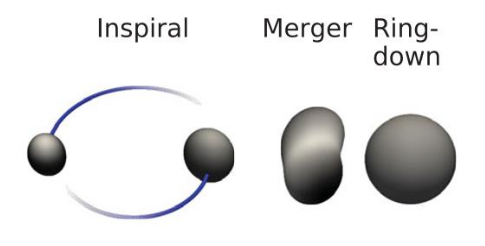
\includegraphics[width=0.5\linewidth]{Images/IMR_figure.png}
    \caption{The three phases of a binary coalescence: inspiral, merger and ringdown.}
    \label{IMR_figure}
\end{figure} 

Note that this is the amplitude as a function of the frequency, so a Fourier transform of $A(t)$.
Here, $f'$ is a frequency ratio using the first transition frequency, see below. 

\begin{equation}
    f'=\frac{f}{f_1}
\end{equation}

The parameter $\nu$ is dimensionless since we are working in geometric units.

\begin{equation}
    \nu=(\pi M f)^(1/3)
\end{equation}

The parameters $\omega_m$ and $\omega_r$ are used to make the function continuous and thus are dependent on the total mass $M=m_1+m_2$. The parameters $\alpha_i$ are post-Newtonian corrections. They are calculated using general relativity and their values are shown in Table \ref{amplitude_param} along with the values for $\epsilon_i$. they are listed with and without the zero-spin approximation which we use in this work.

\begin{table}[h]
    \begin{center}
        \begin{tabular}{ c | c | c | c | c}
            Parameter & $\alpha_2$ & $\alpha_3$ & $\epsilon_1$ & $\epsilon_2$ \\
            \hline
            Value & -323/224 + 451$\eta$/168 & (27/8-11$\eta$/6)$\chi$ & 1.455$\chi$-1.890 & -1.815$\chi$ + 1.656\\
            \hline
            No Spin & -323/224 +  451$\eta$/168 & 0 & -1.890 & 1.656 
        \end{tabular}
        \caption{Amplitude parameters with and without the zero spin approximation.}
        \label{amplitude_param}
    \end{center}
\end{table}

The frequency $f_1$ at the transition of the inspiral and merger phase is the last stable orbit of the binary. Once the merger phase has started the orbits cease to be stable since the objects start to fall in. This corresponds to a maximum of the effective potential. The frequency was calculated by \cite{bardeen_rotating_1972}.

\begin{equation}
    f_1 = \frac{c^3}{6^{3/2}2\pi M_{tot} G}
\end{equation}

The transition frequency from merger to ringdown is given by the least-damped mode (\cite{maggiore_gravitational_2008}) which is also the dominant quasi-normal mode. This is part of the description of the BBH system as characterised by n normal modes with frequencies $\omega_n$, discussed further in chapter 12.3 of the same book.

\begin{equation}
    f_2 \approx 0.747 \frac{c}{2\pi R_S} \approx 12 \rm{kHz} \left( \frac{M_\odot}{M}\right)
\end{equation}

For the ringdown, we have a Lorentzian function $\mathcal{L}$ centred around the merger to ringdown transition frequency $f_2$ with the width $\sigma$.

The global normalisation factor $C$ has the following form in SI units.

\begin{equation}
    C_e = \sqrt{\frac{5}{24}}\frac{(GM_c)^{5/6}}{\pi^{2/3}c^{3/2}}\frac{(1+z)^2}{d_L}
\end{equation}

This depends on the chirp mass which characterises a waveform instead of the total mass and the luminosity distance.

\begin{equation}
    M_c = \frac{(m_1m_2)^{3/5}}{(m_1+m_2)^{1/5}}
\end{equation}

\begin{equation}
    d_L = a_0 (1+z)\int_0^z d\tilde{z}\frac{c}{a_0 H(\tilde{z})}
\end{equation}

\begin{figure}
    \centering
    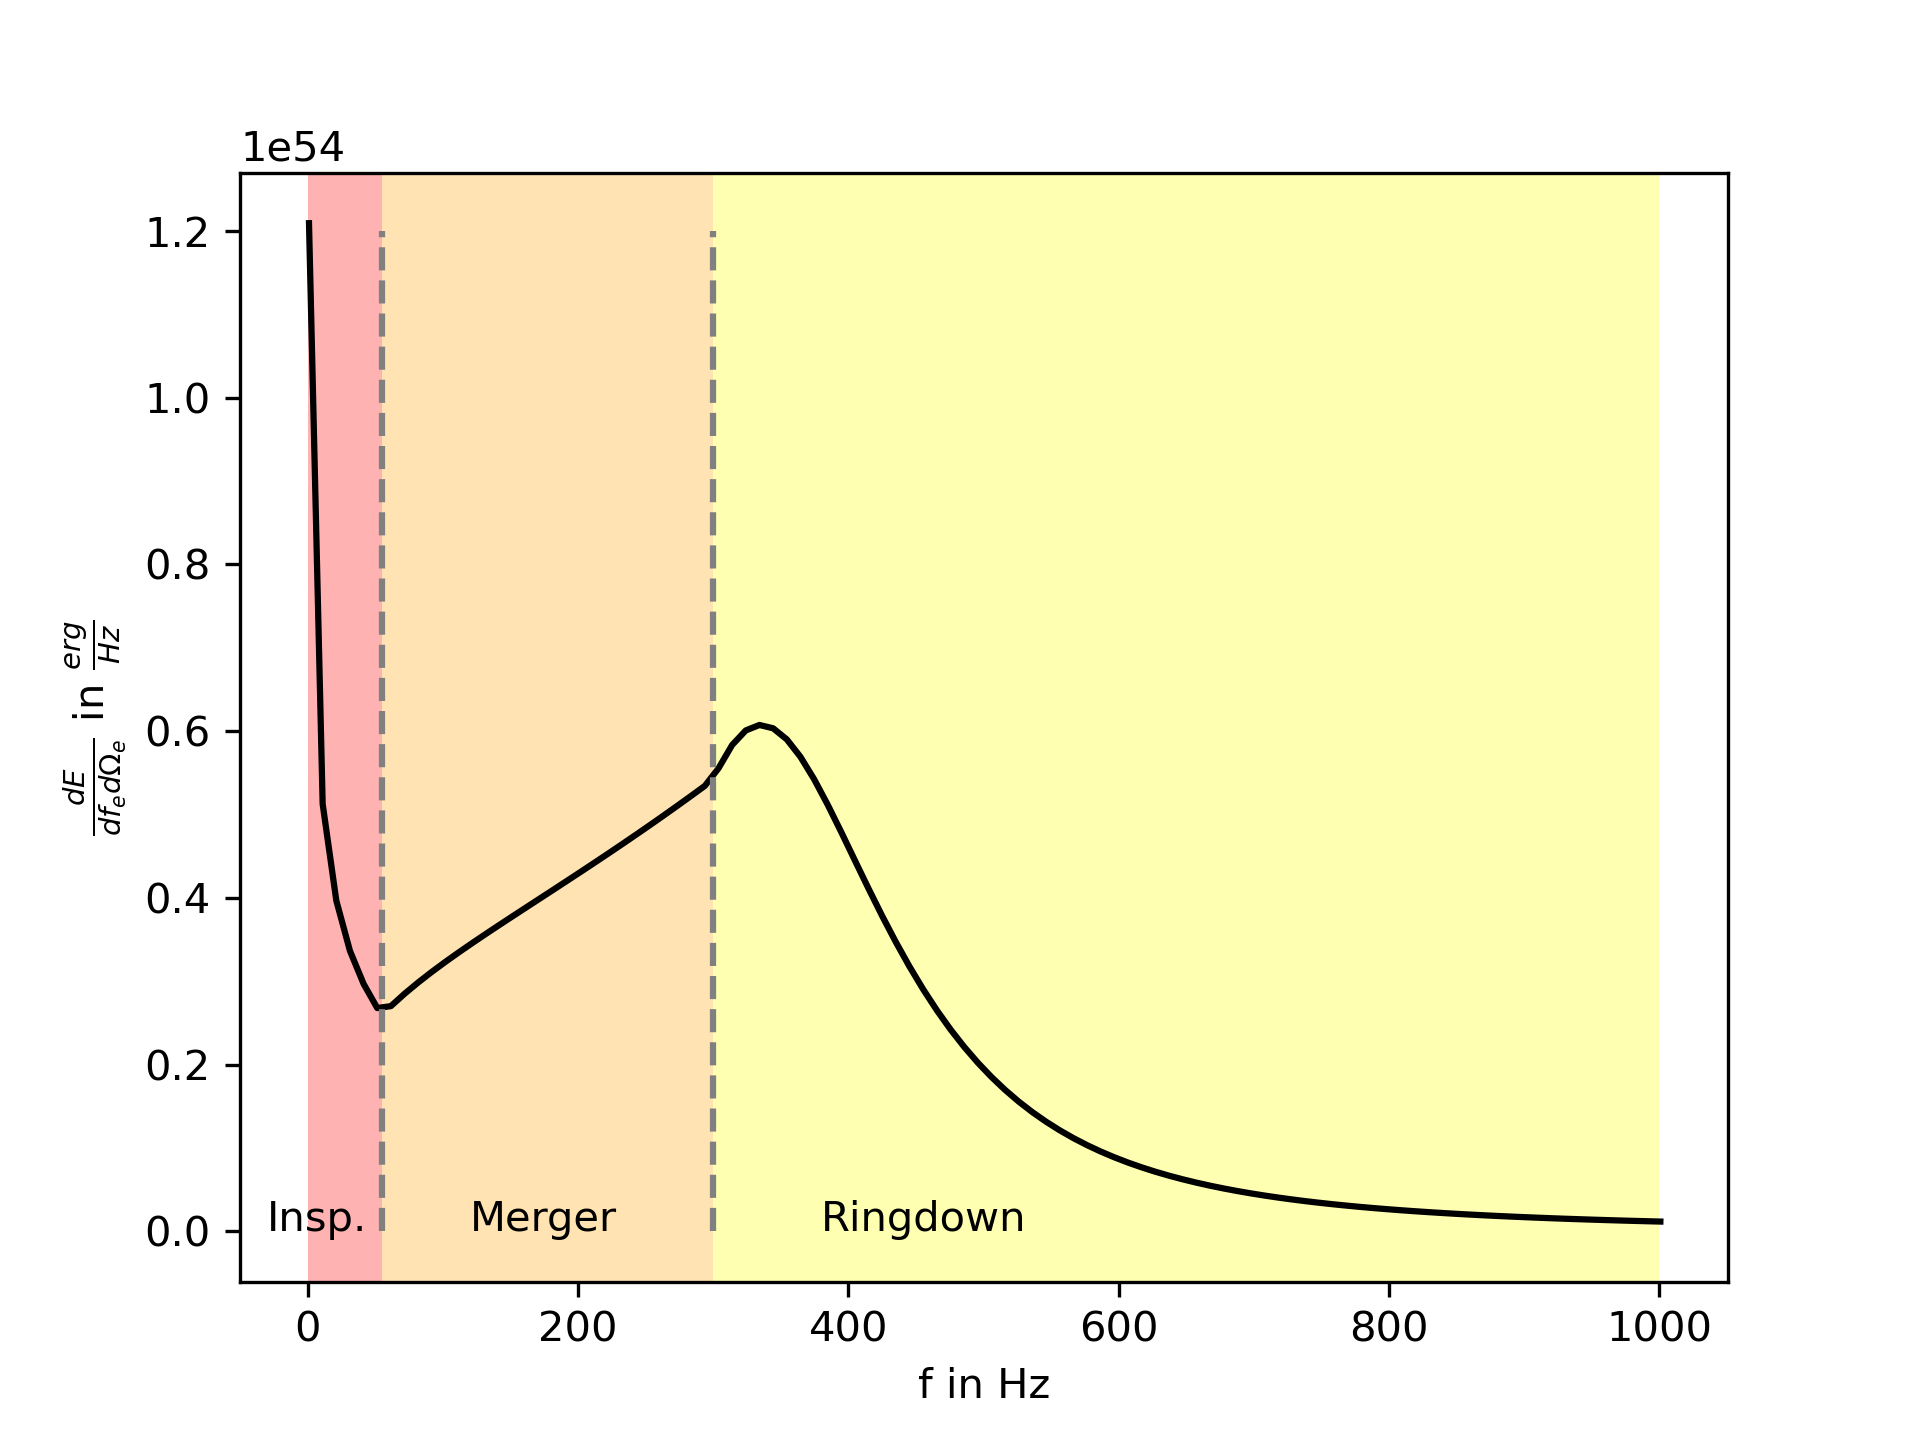
\includegraphics[width=1\linewidth]{Images/dE_df_of_f.png}
    \caption{The energy spectrum as a function of frequency for a BBH merger where both BH have a mass of 20$M_\odot\ $ at $z=0$. }
    \label{dE_df_f}
\end{figure} 


Later, we will consider the square strain as a function of frequency $|h(f)|^2$ for the energy spectrum, so we can ignore the phase $\psi(f)$.

\begin{equation}
    h(f)=A(f)e^{-i\psi(f)}
\end{equation}


Here the redshift dependence will come in through the derivation by the emission 
frequency, see e.g. \ref{window}. From this waveform template, we can get the energy 
spectrum in the following way.
\begin{equation}
    \frac{dE_{GW,e}}{df_e d\Omega_e} = \frac{\pi d_L^2 c^3f_o^2}{2G(1+z)^2} | h(f_o)| ^2 \propto f_o^2h^2(f_o) \propto h^2(t)
\end{equation}


\begin{figure}
    \centering
    \subfloat[1 Hz]{
        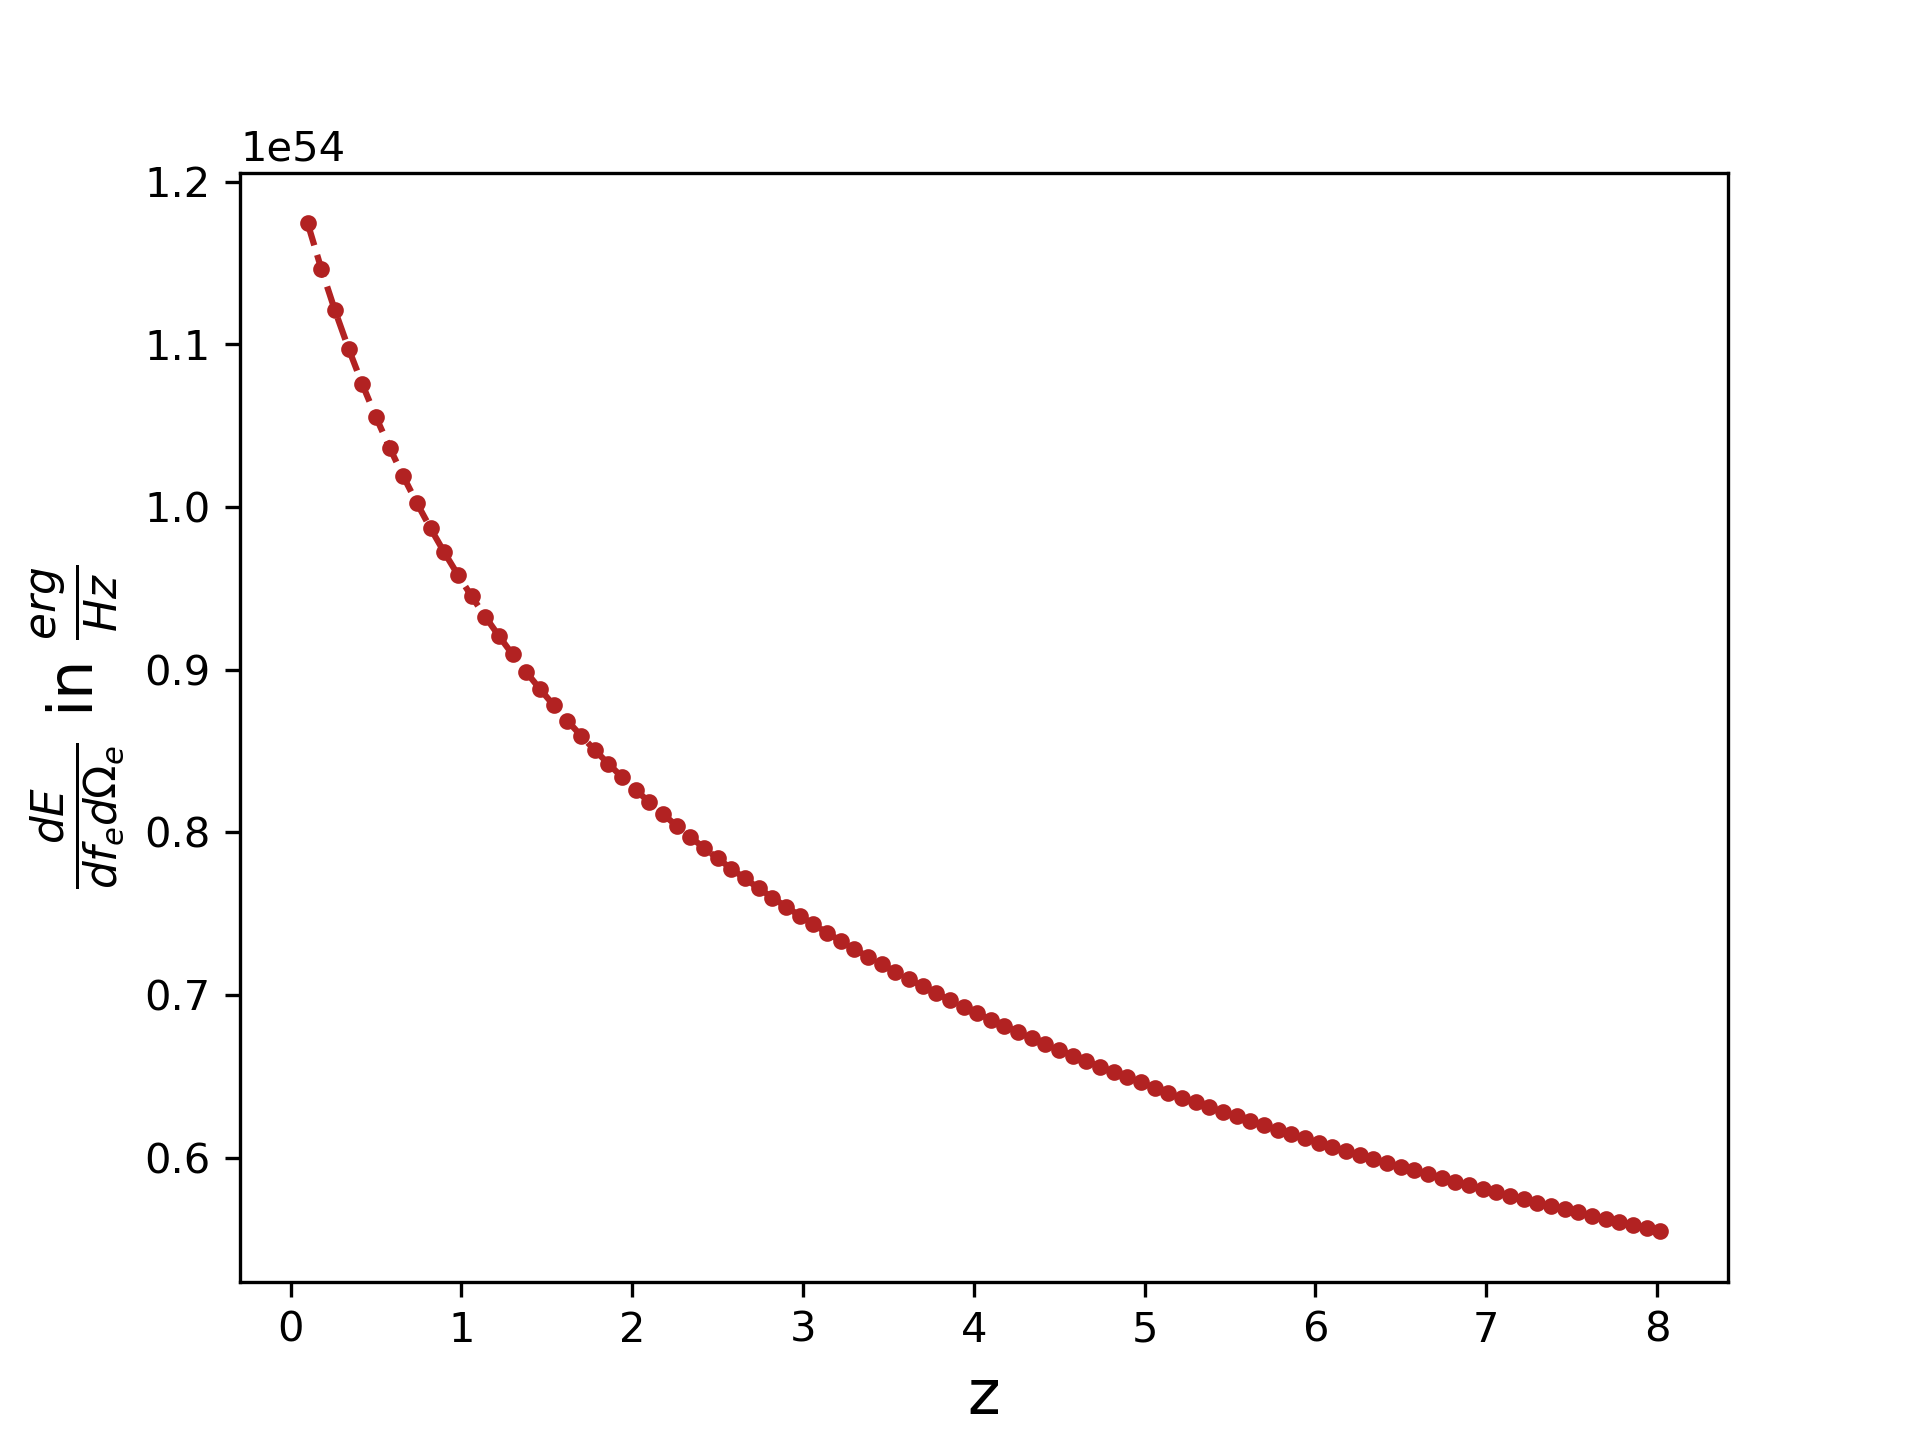
\includegraphics[width=7.5cm, clip]{Images/E_spectrum_z_1Hz.png}}
    %\hspace{1.00\baselineskip}
    \subfloat[10 Hz]{
        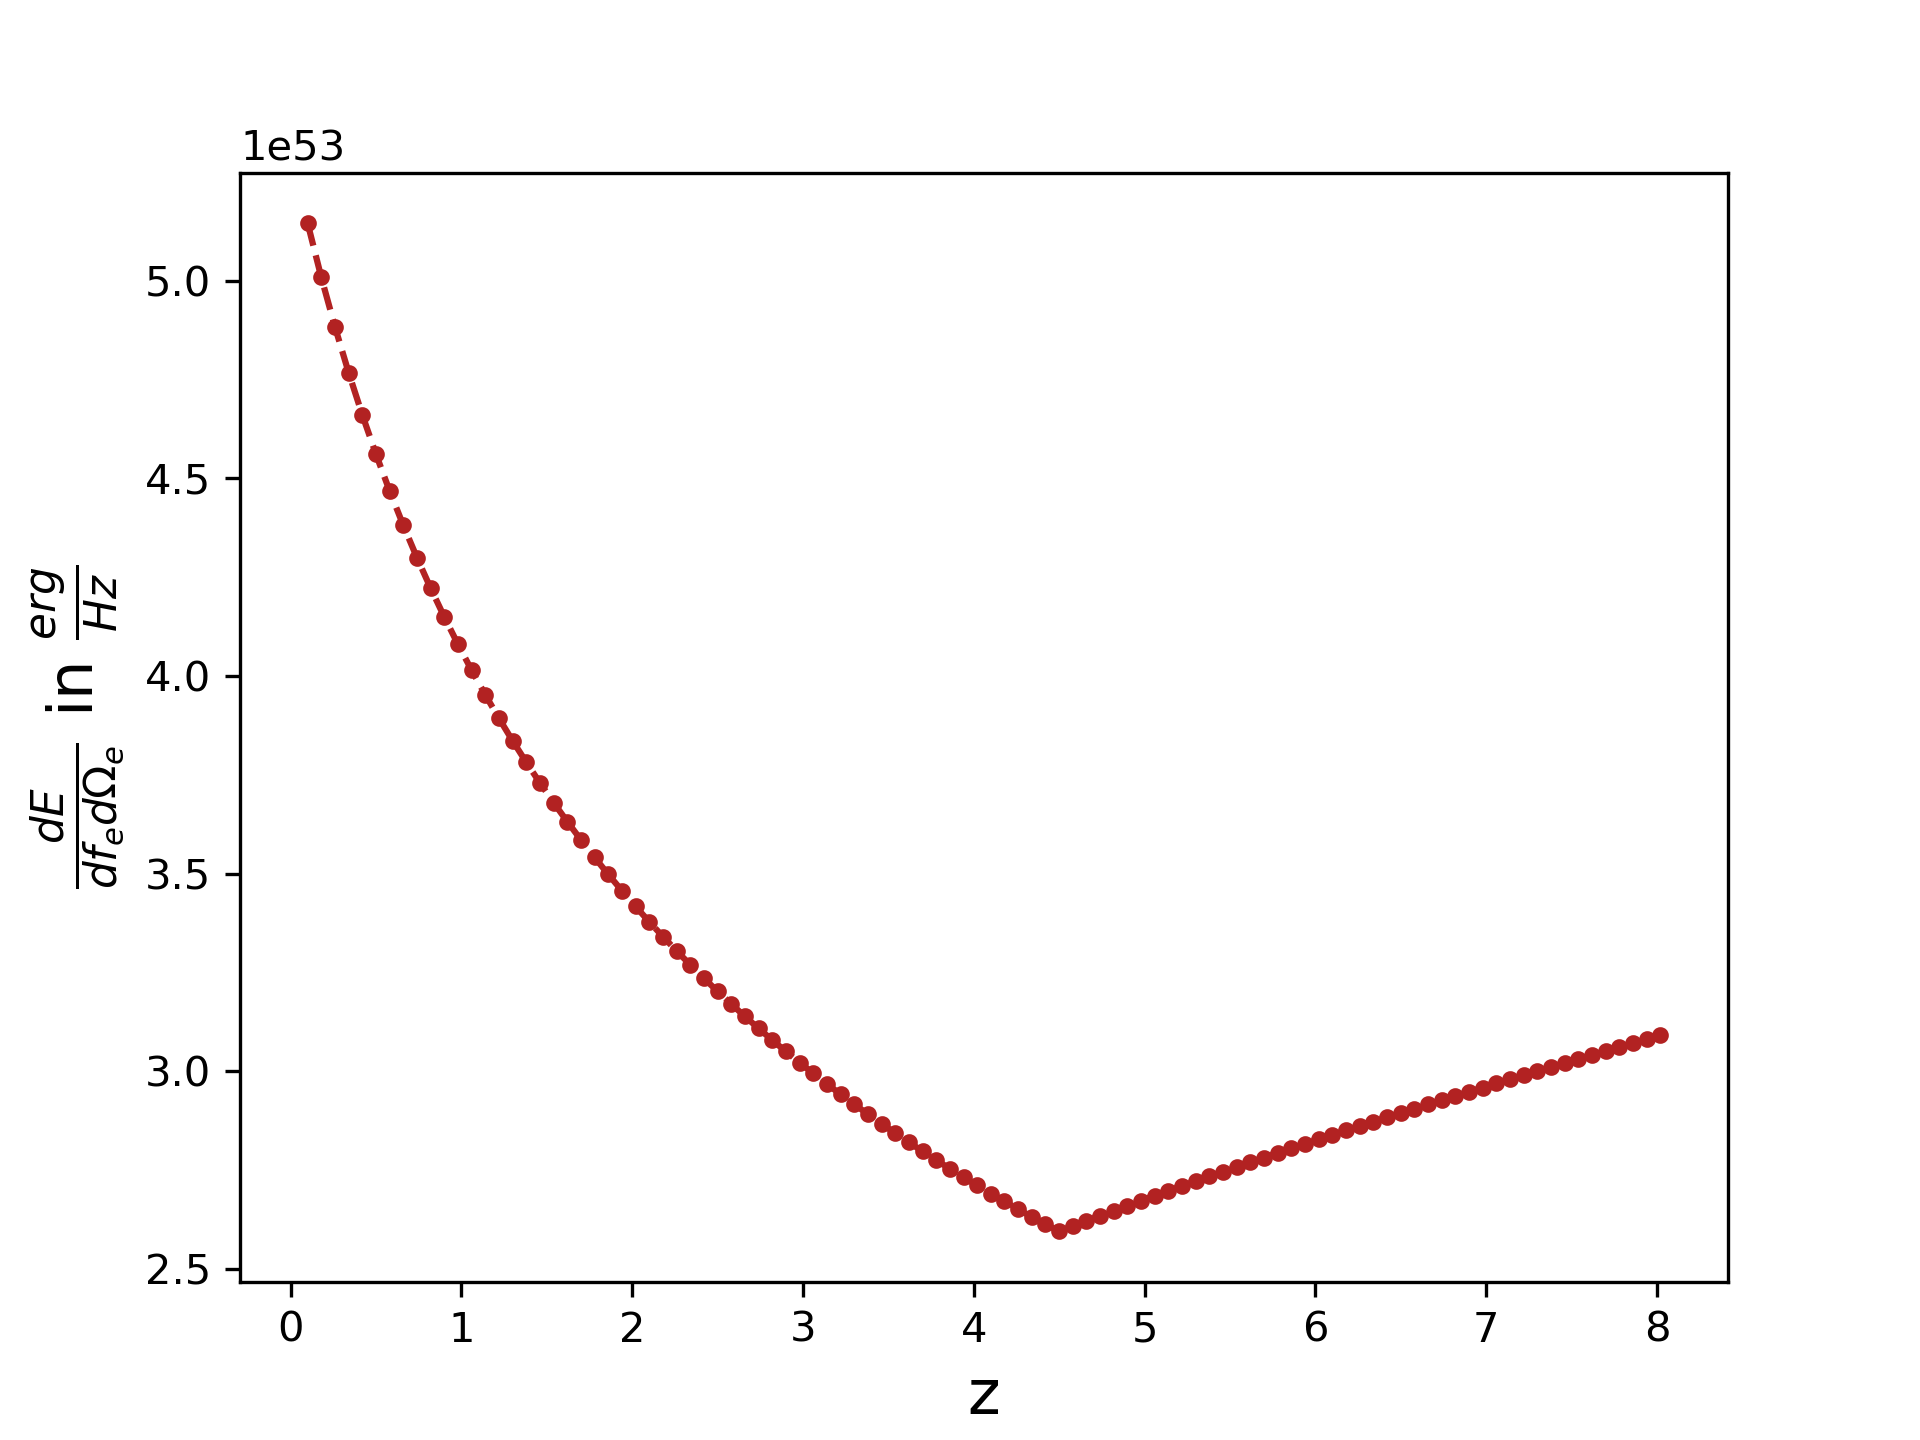
\includegraphics[width=7.5cm, clip]{Images/E_spectrum_z_10Hz.png}}
    \\
    \vspace{-0.5cm}
    \subfloat[100 Hz]{
        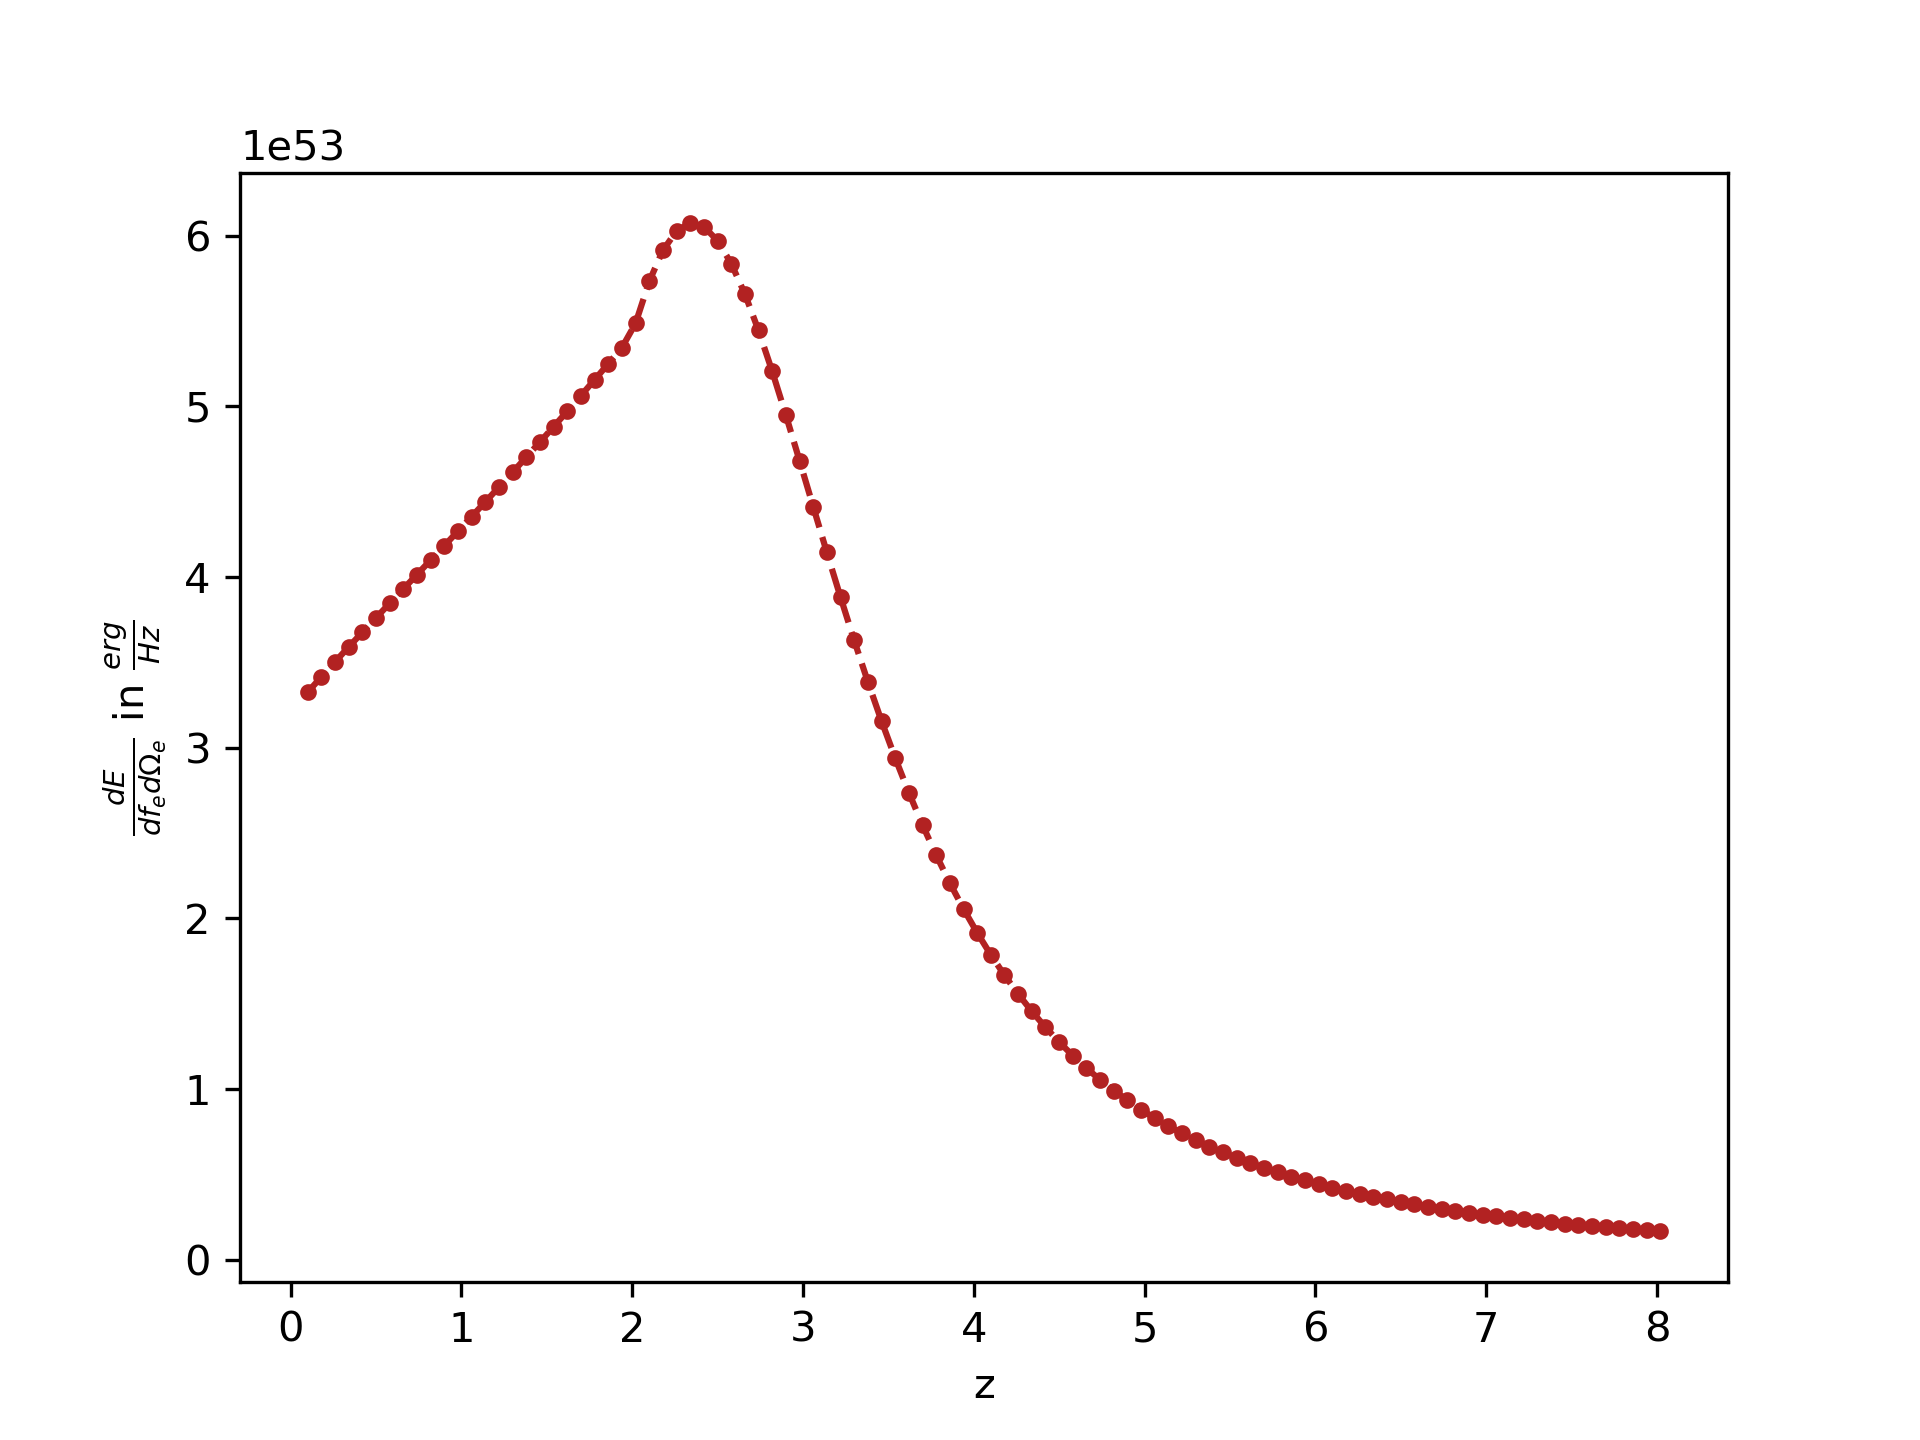
\includegraphics[width=7.5cm, clip]{Images/E_spectrum_z_100Hz.png}}
    %\hspace{-2.00\baselineskip}
    \subfloat[1000 Hz]{
        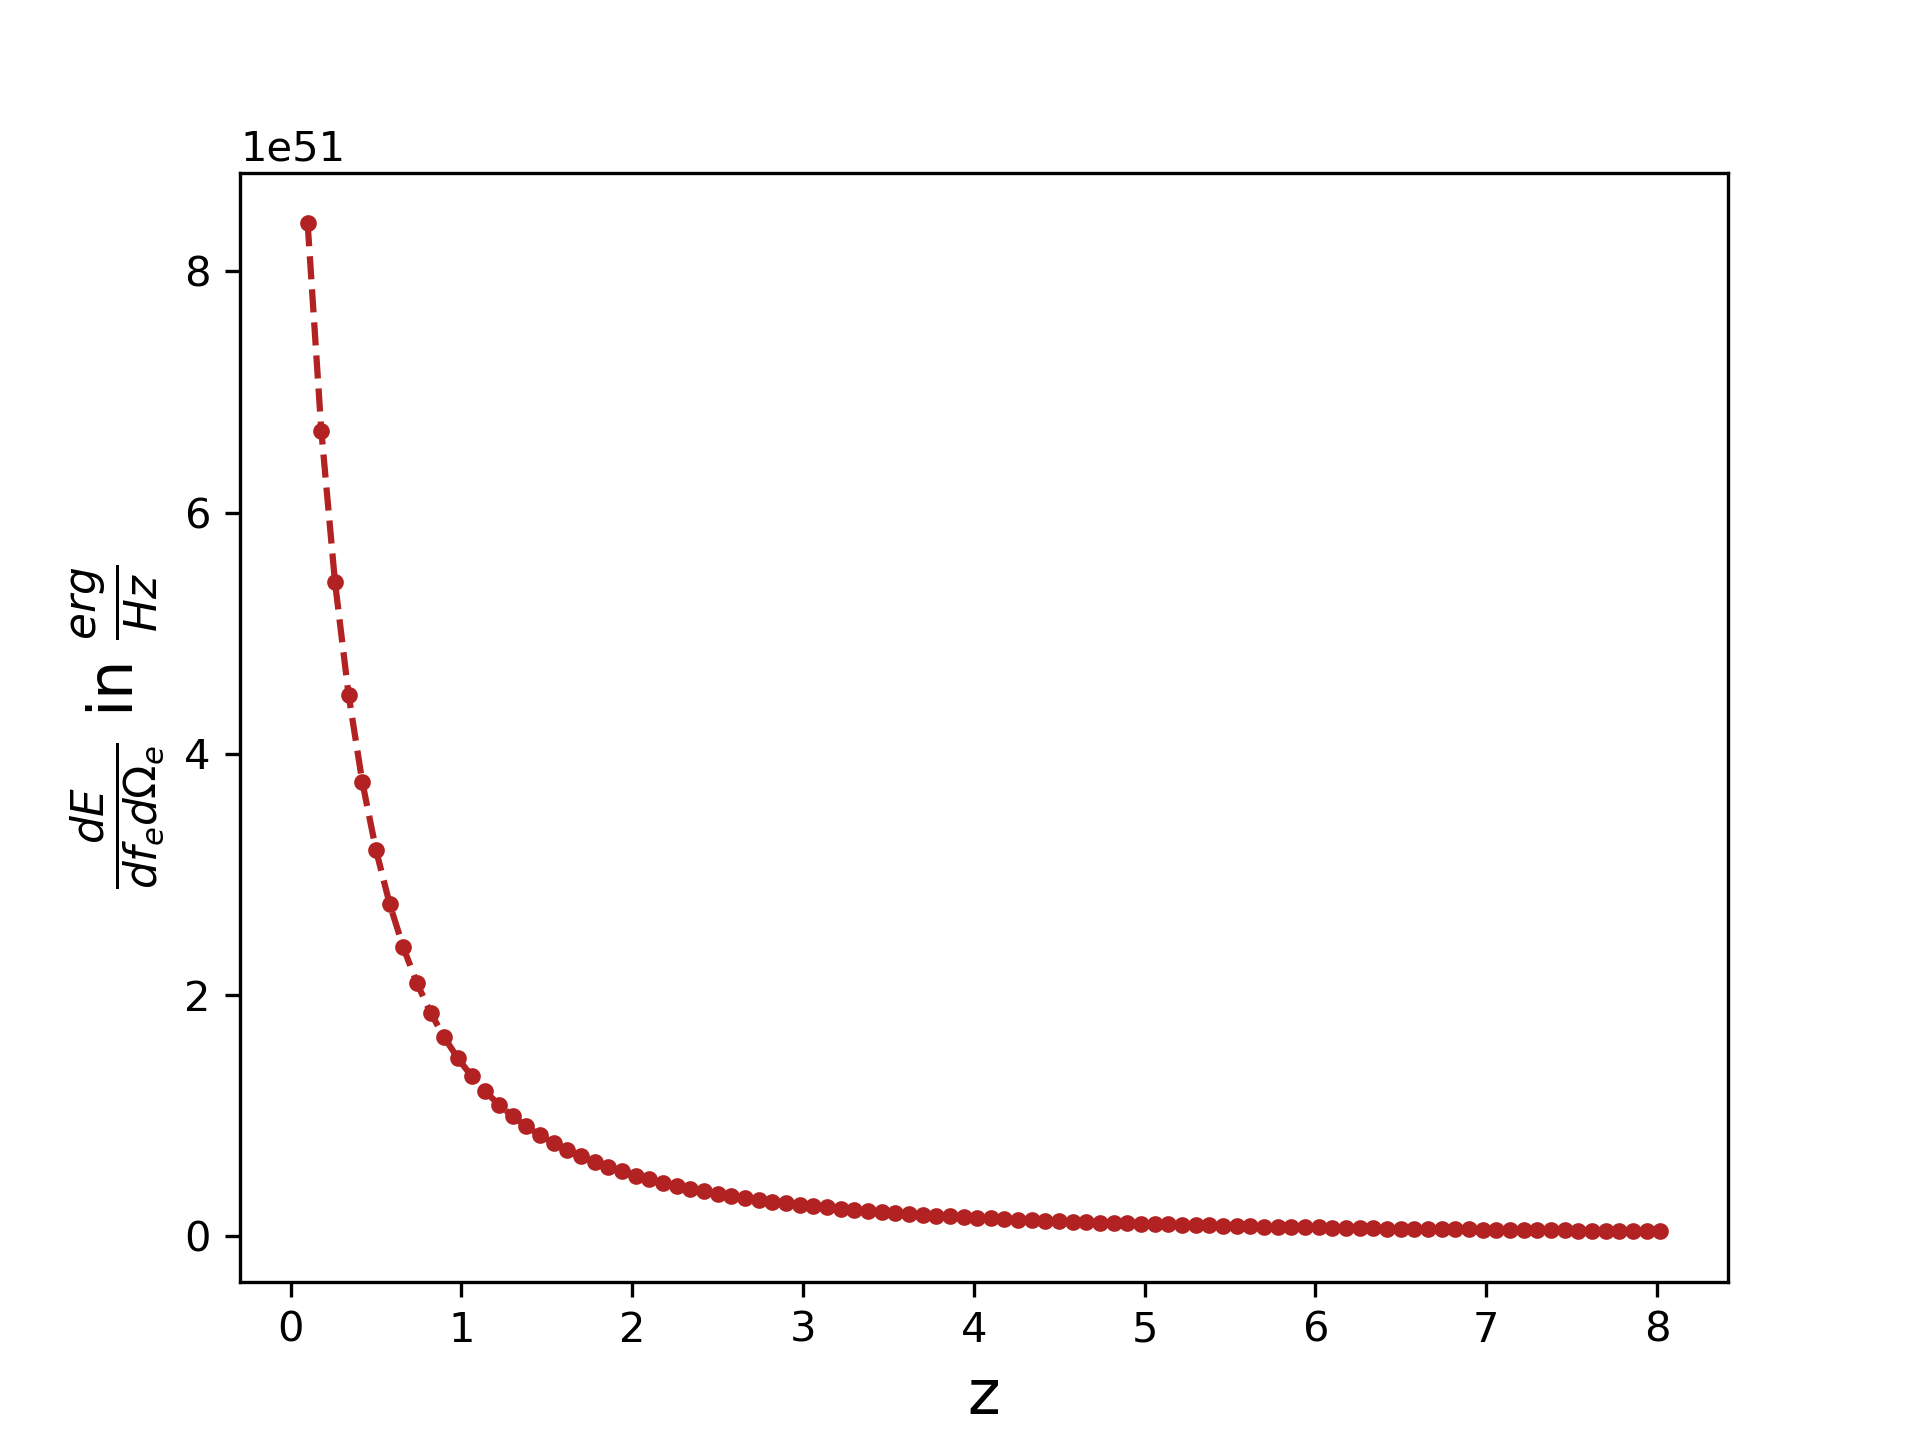
\includegraphics[width=7.5cm, clip]{Images/E_spectrum_z_1000Hz.png}}
  
    \caption{The energy spectrum $d^2 E_{GW,e}/df_e d\Omega_e$ at different observed freqeuncies as a function of redshift.}
    \label{dE_df_diff_frequencies}
\end{figure}

If we plot the energy spectrum as a function of $z$ for different frequencies, see Fig. \ref{dE_df_diff_frequencies}, we can see different sections of Fig. \ref{dE_df_f}. This is because $d^2 E_{GW,e}/df_e d\Omega_e$ only depends on z through the emitted frequency. The energy spectrum is written as a function of $f_e$, but we implement it in such a way that the user can choose the received frequency at the detector.

\begin{equation}
    f_e = (1+z)f_0
\end{equation}

At lower frequencies, like 1 Hertz, the energy spectrum consists of the inspiral phase. At 10 Hertz, we can see the transition from the inspiral to the merger phase. The transitions are not always smooth since the parameters $\omega_i$ fix the continuity of the curve but not the slope. The transition to the ringdown is visible at 100 Hertz. At high frequencies such as 1000 Hertz, the ringdown phase dominates at all redshifts.

To speed up the calculation, we assume $m_1 = m_2 = 20M_\odot$. This is a common BH mass considering GW observations from LVK \cite{the_ligo_scientific_collaboration_population_2022}.

\section{Star Formation Rate}

The BBH merger rate depends on the star formation rate (SFR) which is the rate at which gas and dust are turned into stars. This is relevant since BH are end products of stellar evolution.

\begin{equation}
    R_{BBH}(z) \propto \int dM_h \frac{dn}{dM_h}(z_f, M_h)\langle SFR(M_h, z_f)\rangle_{SF}
\end{equation}


For the star formation rate, we use the \textsc{UniverseMachine} code from \cite{behroozi_universemachine_2019}. They use observational constraints and data from simulations to compute SFR for individual galaxies.

In the $\Lambda$CDM cosmology, galaxies form at the centre of haloes. Haloes are gravitationally self-bound structures that contain virialised dark matter. This means that the virial equation applies in this case. Here, $T$ is the potential energy and $U$ is the kinetic energy.

\begin{equation}
    2T=U
\end{equation}

So far, there exists no framework in which we can derive the SFR from first principles. This is why the authors use a double power law plus Gaussian and determine the best-fit parameters for this functional form. This determines the SFR for every halo at a given redshift. They use weak priors and observational constraints for less bias and the potential to reveal new physics.

Dark matter simulations, here Bolshoi-Planck [\cite{klypin_dark_2011}] and MultiDark Planck 2 (MDPL2) \cite{klypin_multidark_2016}, are used, which simulate a mock universe. They contain halo merger trees, which can be compared to observations. Behroozi et al. used data from multiple experiments, such as the Sloan Digital Sky Survey (SDSS) \cite{abazajian_seventh_2009}, Ultravista \cite{mccracken_ultravista_2012}. The observables include stellar mass functions, UV luminosity functions and galaxy auto-correlation functions.
Using this data, they compute a likelihood and run a Markov Chain Monte Carlo (MCMC) algorithm to sample the SFR range.

Like in \cite{dallarmi_dipole_2022} we consider only star-forming galaxies. This could be modified in a future version of the code by including the fraction of quenched galaxies $f_Q = 1 -f_{SF}$, which could be taken from the \textsc{UniverseMachine} paper as well. The adopted SFR functional form is the following. The fit parameters depend on the rotational velocity at peak halo mass $v_{Mpeak}$ and on the redshift. This velocity only depends on the halo mass $M_h$, see below.

\begin{equation}
    \langle SFR_{SF}(M_{peak}(v_{Mpeak, z}), z)\rangle = \epsilon \left[ \left( v^\alpha + v^\beta \right)^{-1} + \gamma \exp \left(-\frac{\log_{10}(v)^2}{2\delta^2}\right) \right]
\end{equation}

The characteristic SFR  in $M_\odot\ yr^{-1}$ is the global factor $\epsilon$. For the slope of the $SFR-v_{Mpeak}$ relation, we have a faint-end and a massive-end slope parameter $\alpha$ and $\beta$, respectively. This is because $v_{Mpeak} \propto M_h^3$ \ref{v_mpeak-M_h-relation}, so a higher velocity at the peak mass corresponds to a higher halo mass.
Furthermore, $\gamma$ is the strength and $\delta$ the width of the Gaussian SFR efficiency boost. 

The velocity $v$ is defined as the ratio of the real ($v_{Mpeak})$ and the characteristic ($V$) velocity at the halo peak mass, both in $km s^{-1}$.

\begin{equation}
    v = \frac{v_{Mpeak}}{V \cdot km s^{-1}}
\end{equation}



\begin{figure}
    \centering
    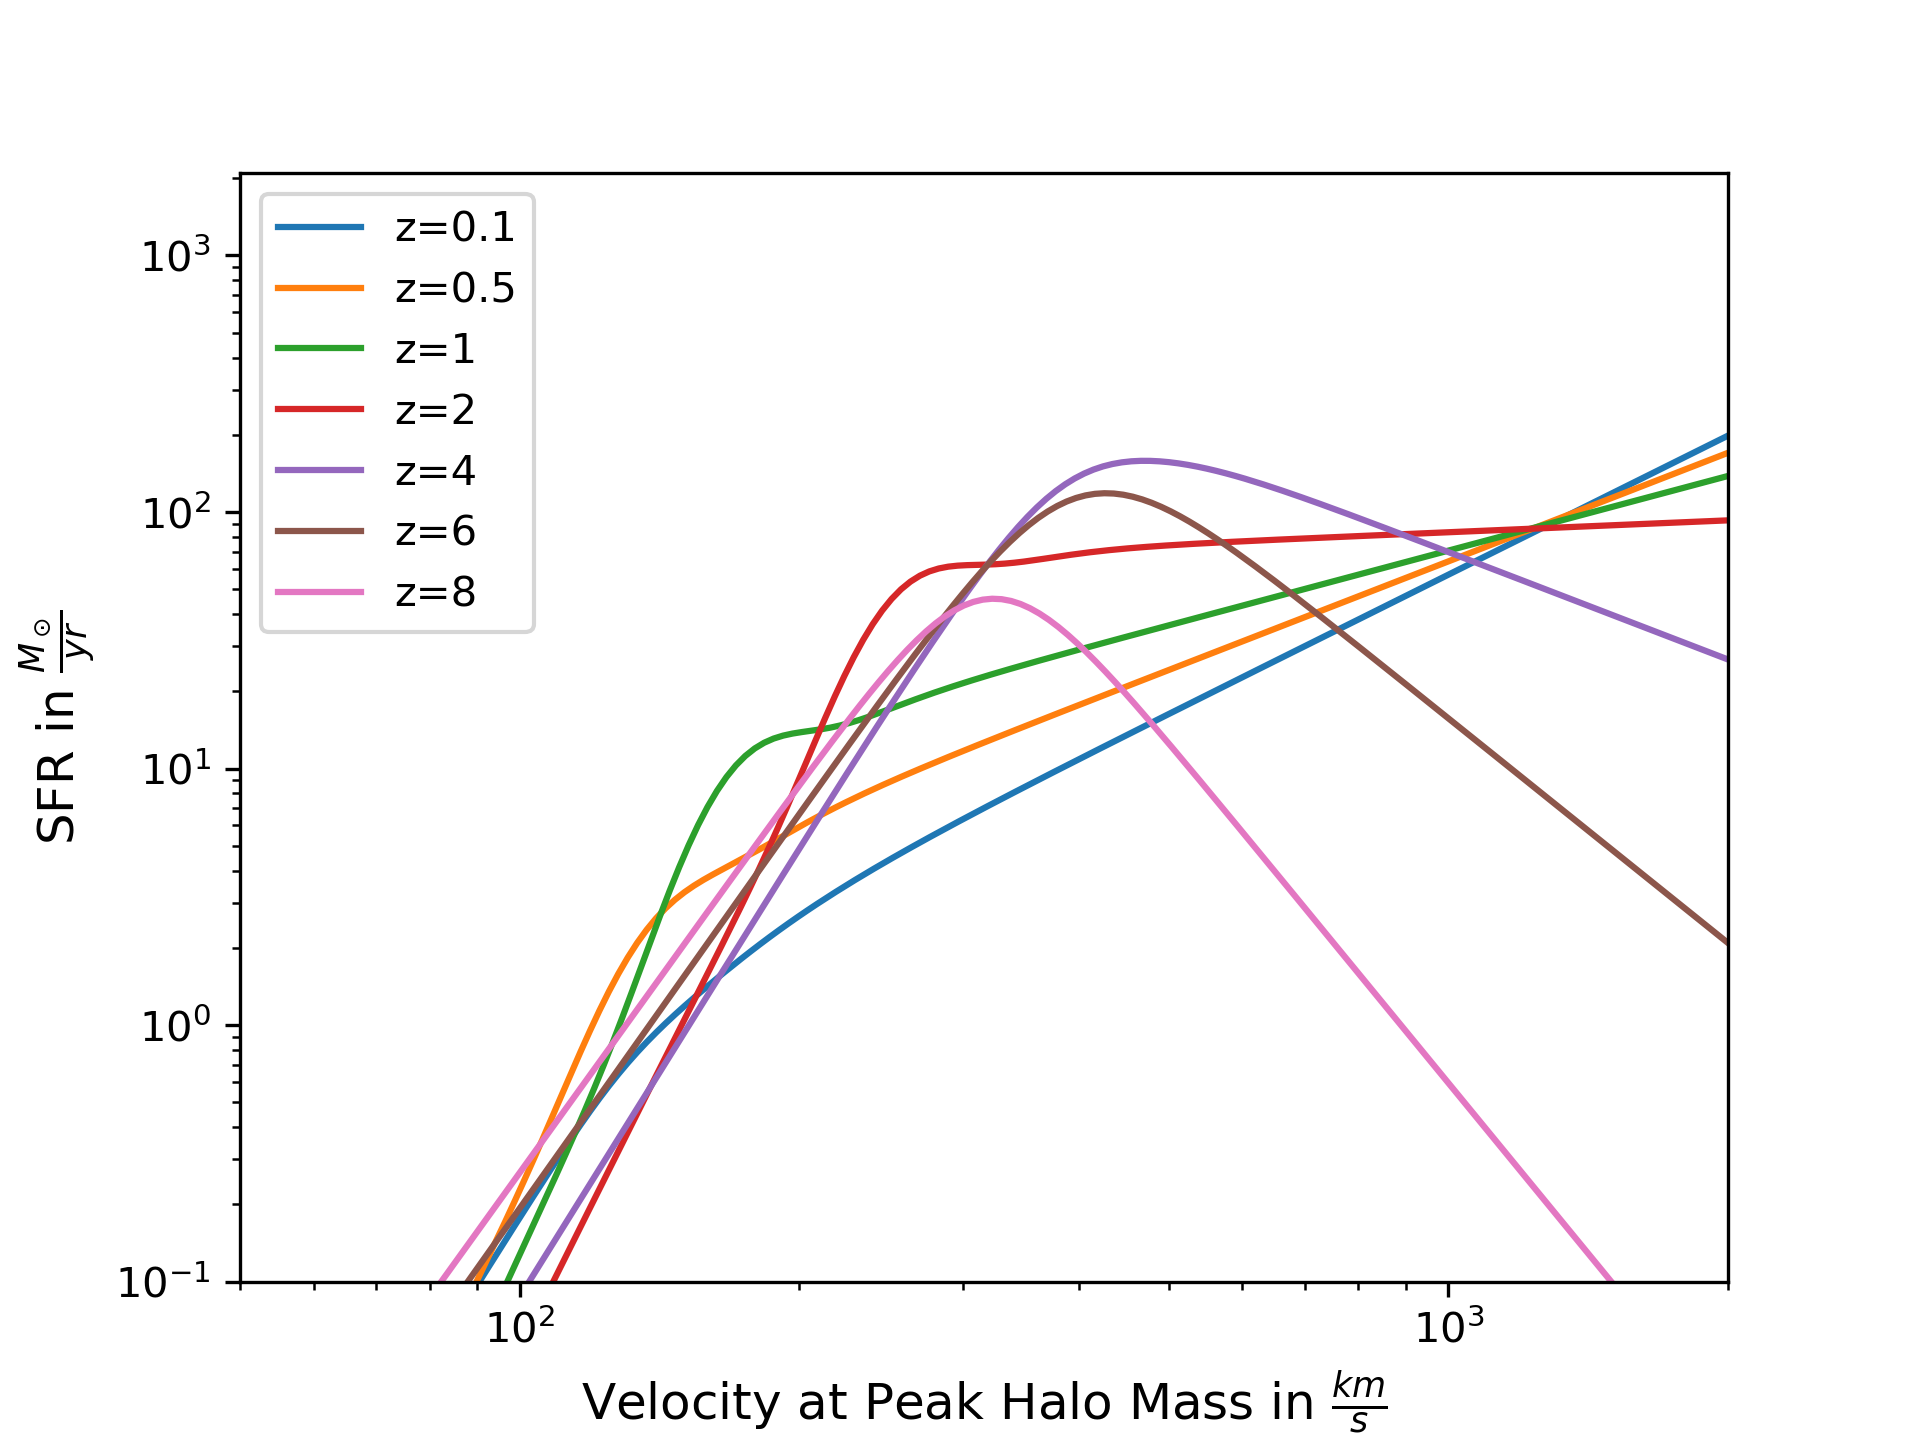
\includegraphics[width=1\linewidth]{Images/sfr_of_v.png}
    \caption[The SFR for star-forming galaxies for different redshifts.]{The SFR for star-forming galaxies for different redshifts. The velocity at the historical peak halo mass corresponds to the standard halo mass, see equation \ref{v_mpeak-M_h-relation}.}
    \label{SFR_of_v}
\end{figure} 

The other parameters, except for $\delta$, scale differently for different redshift regions. For $V$, $\epsilon$ and $\alpha$, the scaling is separated into $z=0$, $z\approx 1-2$, $z=3-7$ and $z>7$. The parameters $\beta$ and $\gamma$ have three scaling regions instead of four, as they are not well constrained at high redshifts. 

\begin{equation}
    \log_{10}(V) = V_0 + V_a(1-a)+V_{la}ln(1+z)+V_z z
\end{equation}
\begin{equation}
    \log_{10}(\epsilon) = \epsilon_0 + \epsilon_a(1-a)+\epsilon_{la}ln(1+z)+\epsilon_z z
\end{equation}
\begin{equation}
    \alpha = \alpha_0 + \alpha_a(1-a)+\alpha_{la}ln(1+z)+\alpha_z z
\end{equation}
\begin{equation}
    \beta = \beta_0 + \beta_a(1-a)+\beta_z z
\end{equation}
\begin{equation}
    \log_{10}(\gamma) = \gamma_0 + \gamma_a(1-a)+\gamma_{la}ln(1+z)+\gamma_z z
\end{equation}
\begin{equation}
    \delta = \delta_0
\end{equation}



The median $v_{Mpeak}$ is taken from the \textit{Bolshoi-Planck} DM simulation as

\begin{equation}
    v_{Mpeak}(M_h, a) = 200 \frac{km}{s}\left[ \frac{M_h}{M_{200kms}(a)}\right]^3
    \label{v_mpeak-M_h-relation}
\end{equation}
\begin{equation}
    M_{200kms}(a) = \frac{1.64 \cdot 10^{12} M_\odot\ }{()\frac{a}{0.378})^{-0.142}+(\frac{a}{0.378})^{-1.79}} .
\end{equation}

\section{Halo Mass Function}

The merger rate of BBH depends on the number of haloes since their formation takes place in haloes. This is why it depends on the halo mass function (HMF) $\frac{dn}{dM_h}(z_f, M_h)$ integrated over the halo mass. 
\begin{equation}
    R_{BBH}(z) \propto \int dM_h \frac{dn}{dM_h}(z_f, M_h)\langle SFR(M_h, z_f)\rangle_{SF}
\end{equation}

The HMF is the comoving number density of haloes with masses between $M$ and $M+dM$. 

We first consider the variance of the matter density field $\sigma^2$ which we get from the linear matter power spectrum integrated over the wavenumber $k$ with a window function. This is the Fourier transform of a tophat function in real space with the width $R$, corresponding to the radius of the spherical halo. Physically, overfull regions in the universe gravitationally attract and form haloes.

\begin{equation}
    \sigma^2(R, z) = \int_0^\infty k^2 P_{lin}(k, z) W^2(k, R) dk
\end{equation}

For a spherical halo model, we get the radius through the mass and the density.

\begin{equation}
    R= \sqrt[3]{\frac{3M}{4\pi \rho_m}}
\end{equation}

Then, the halo mass function comes from the logarithmic derivative of $\sigma^{-1}$ by the halo mass.

\begin{equation}
    \frac{dn(M)}{dM }=\frac{\rho_m}{M^2}\frac{d\ln (\frac{1}{\sigma})}{d\ln M}f_{NL}(\sigma)
\end{equation}

The factor $f_{NL}$ accounts for non-linear effects in the halo collapse. There are different ways to model these effects. A common analytical one is the Press-Schechter formalism parametrised by the critical overdensity $\delta_c$.

\begin{equation}
    \delta = \frac{\delta \rho}{\bar{\rho}}
\end{equation}

\begin{equation}
    f_{PS}(\sigma)=\sqrt{\frac{2}{\pi}} \frac{\delta_c}{\sigma}\exp(-\frac{\delta_c^2}{2\sigma^2})
\end{equation}

Here, we use the parametrisation by \cite{tinker_toward_2008}. They use a fitting formula depending on the overdensity $\Delta$. The overdensity characterises how much denser the halo is compared to the average universe density $\bar{\rho}_m$ at the corresponding redshift.

\begin{equation}
    \Delta = \frac{3M_{\Delta}}{4\pi R^3_{\Delta}\bar{\rho_m}}
\end{equation}

The non-linear corrections then have the following form.

\begin{equation}
    f(\sigma)=A \left( \left(\frac{\sigma}{b}\right)^{-a}+1\right)\exp(-\frac{c}{\sigma^2})
\end{equation}

The used fitting parameters, dependent on the overdensity, are the following.

\[ A = \begin{cases}
    0.1(\log_{10}\Delta)-0.05 & \Delta<1600 \\
    0.26 & \Delta \geq 1600
\end{cases}
\]

\begin{equation}
    a=1.43+(\log_{10}\Delta -2.3)^{1.5}
\end{equation}
\begin{equation}
    b=1.0+(\log_{10}\Delta -1.6)^{-1.5}
\end{equation}
\begin{equation}
    c=1.2+(\log_{10}\Delta -2.35)^{1.6}
\end{equation}

To show how the redshift and the overdensity influence the HMF, we vary the parameter in Fig. \ref{HMF_delta}.

\begin{figure}
    \centering
    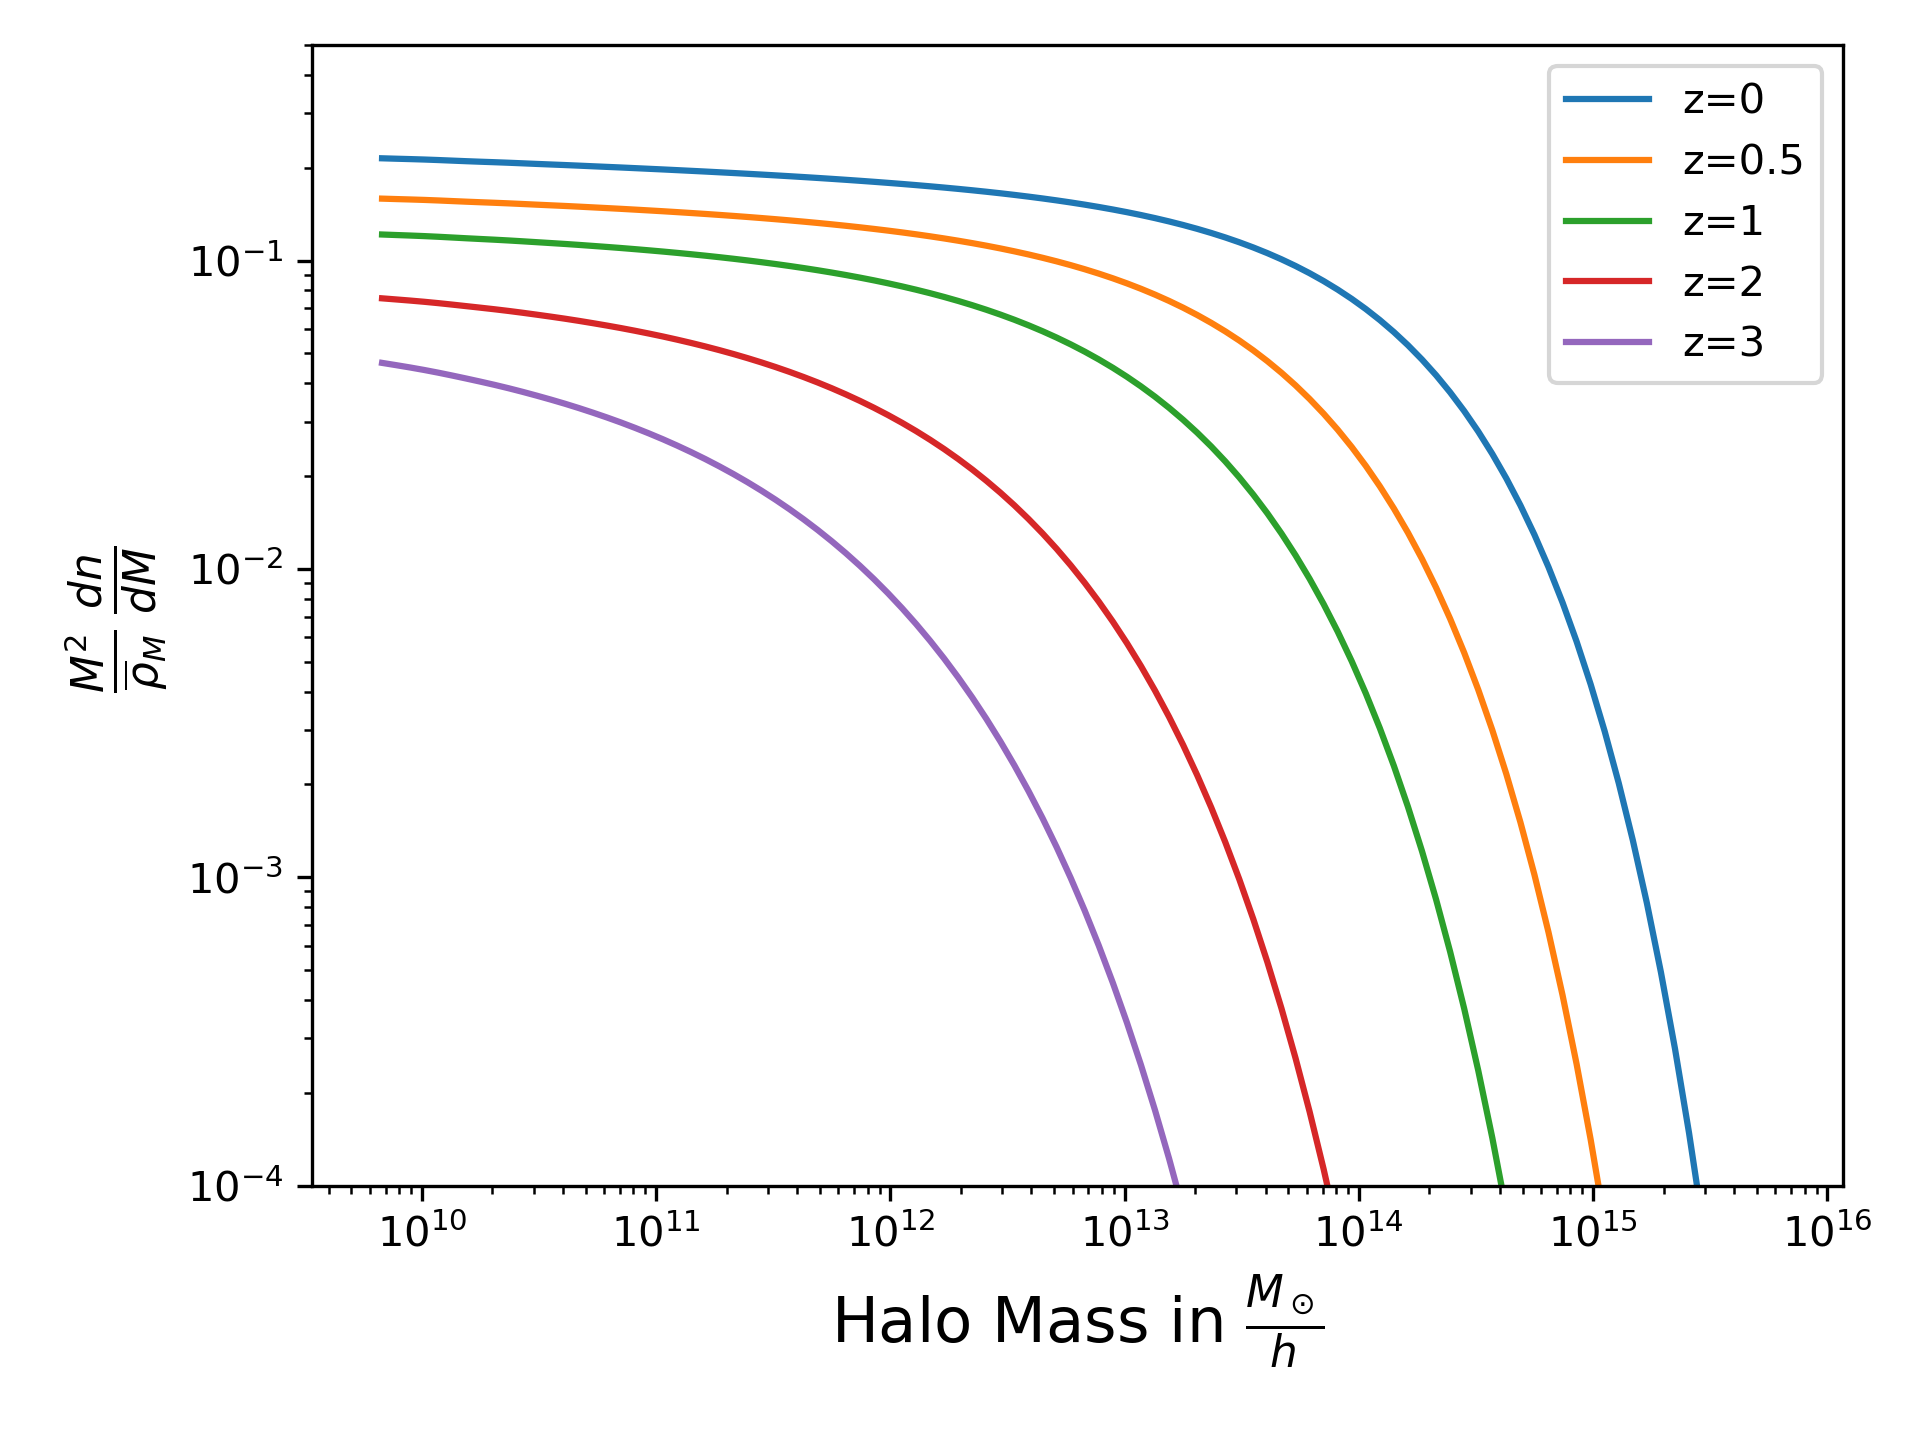
\includegraphics[width=0.9\linewidth, clip]{Images/HMF_diff_z.png}
    \caption{The dimensionless HMF for different redshifts $z$ at $\Delta=800$.}
    \label{HMF_z}
\end{figure} 

\begin{figure}
    \centering
    \subfloat[{The dimensionless HMF for different overdensity parameters $\Delta$ at $z=0$.}
        \label{HMF_delta}]{
        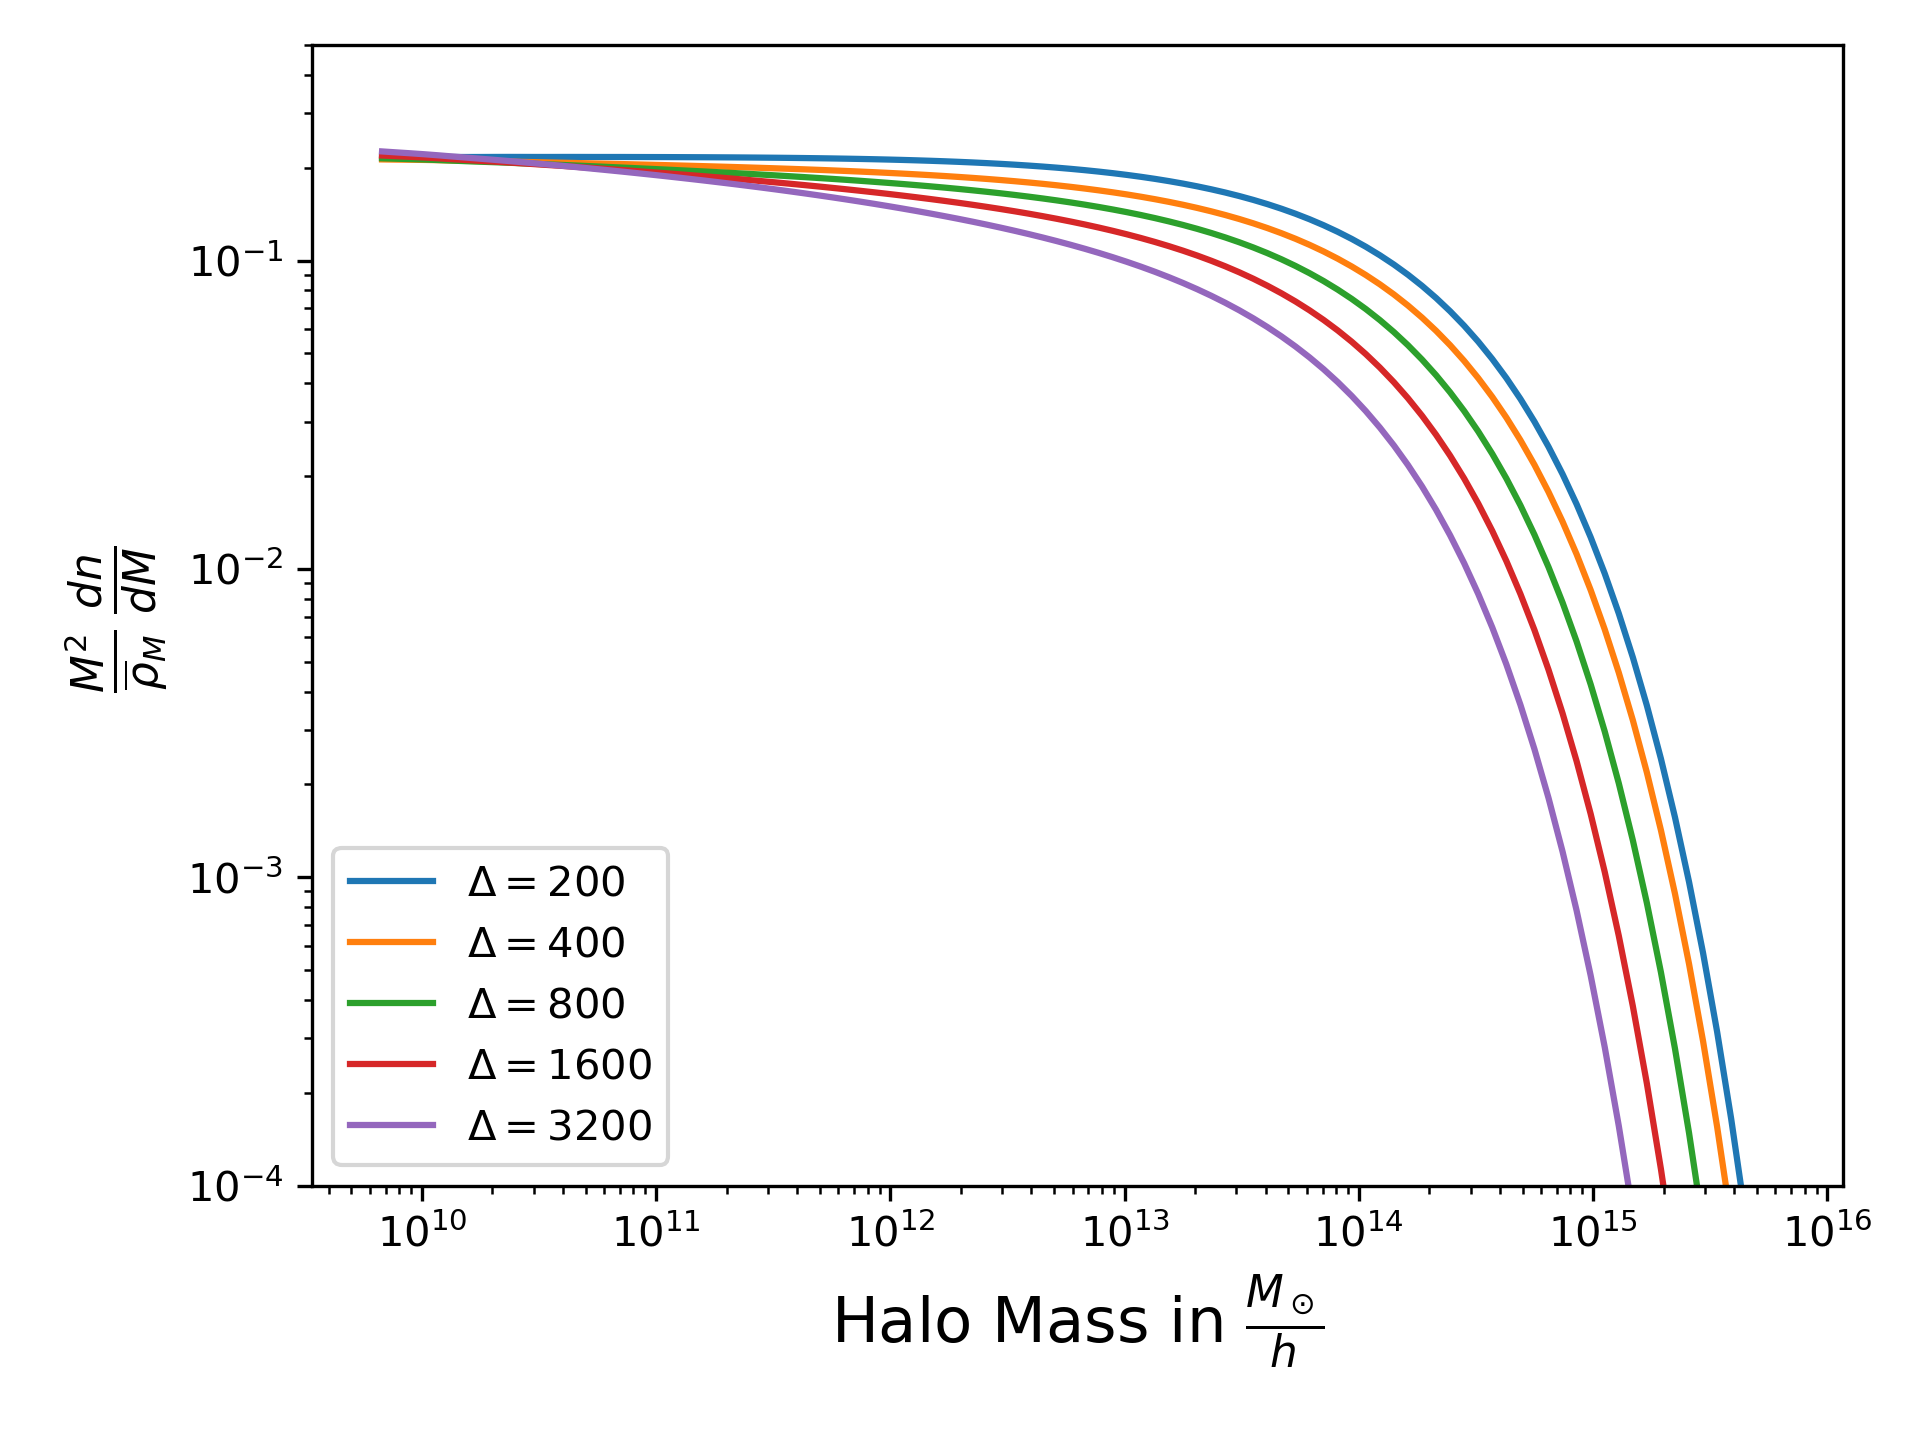
\includegraphics[width=7.5cm, clip]{Images/HMF_diff_delta.png}}
    \subfloat[The HMF in units of $\frac{h/M_\odot}{(Mpc/h)^3}$ or respectively $\frac{h^4}{M\odot Mpc^3}$ with $\Delta=800$, here at $z=0$.
        \label{HMF_dim}]{
        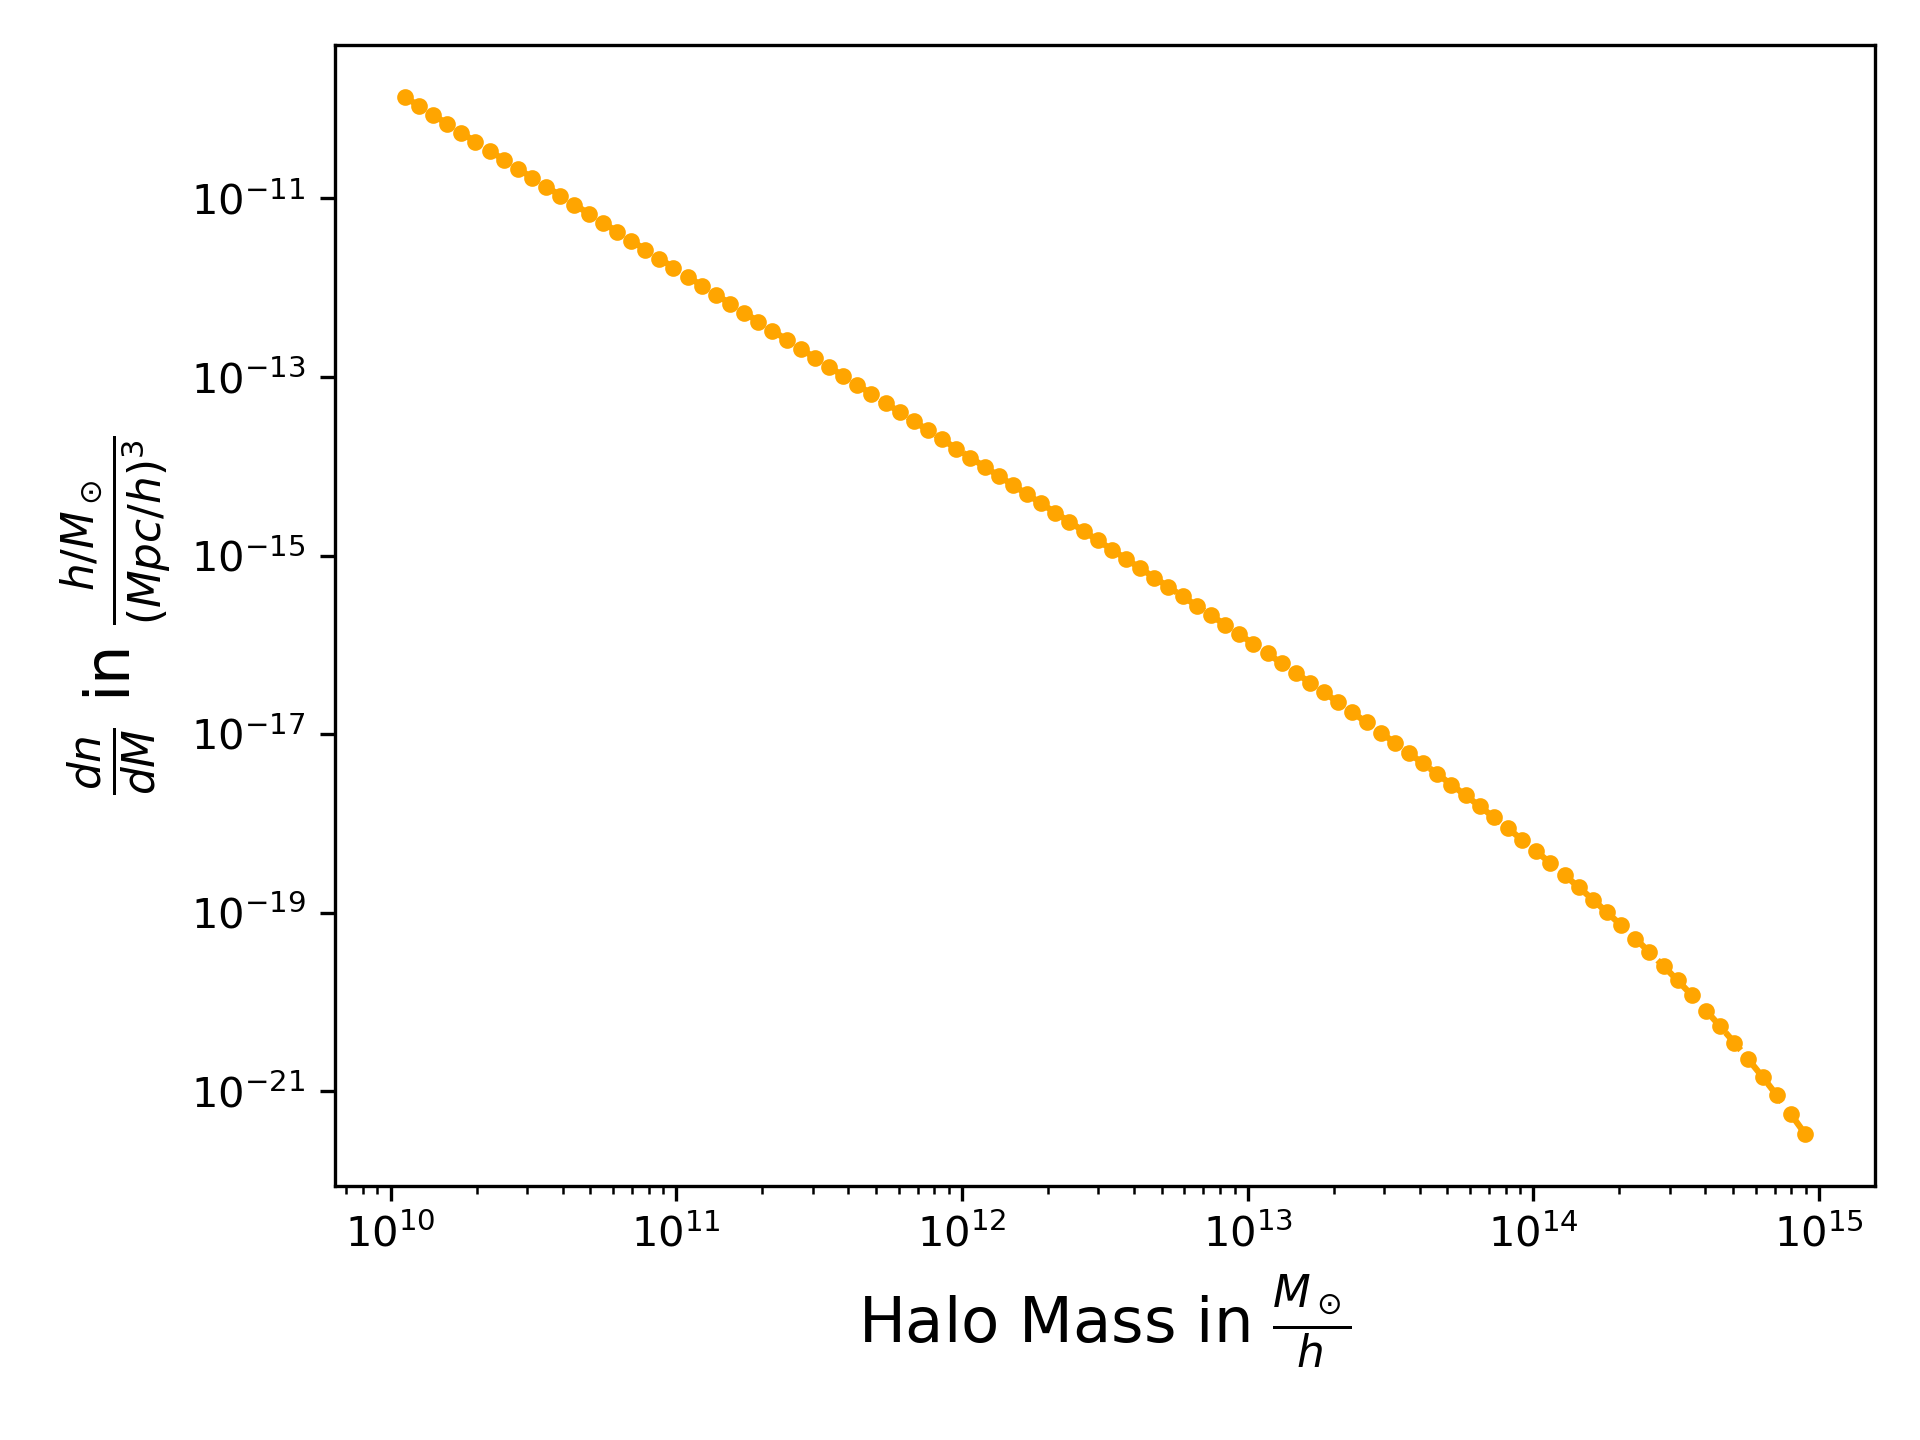
\includegraphics[width=7.5cm, clip]{Images/HMF.png}}
    \caption{The HMF at $z=0$.}
\end{figure} 

\section{Merger Rate}

With the SFR and the HMF, we can now calculate the BBH merger rate.
\begin{equation}
    R_{BBH}(z=0) = 19 \:\rm{Gpc}^{-3}\rm{yr}{-1}
\end{equation}
\begin{equation}
    R_{BBH}(z)=\mathcal{A}_{LIGO}^{BBH}\int dt_d p(t_d) \int dM_h \frac{dn}{dM_h}(z_f, M_h)\langle SFR(M_h, z_f)\rangle_{SF}
    \label{BBH_merger_equation}
\end{equation}

Here, we have the time delay distribution $p(t_d)$, where the time delay takes place between the formation and the merger of the binary. 

\begin{equation}
    p(t_d)=\ln\left(\frac{t(z)}{t_{d, min}}\right)\frac{1}{t_d}
\end{equation}

The minimum time delay is 50 Myr, like in \cite{dallarmi_dipole_2022}. 

The merger rate is also multiplied by a normalisation factor $\mathcal{A}_{LIGO}^{BBH}$, corresponding to the local merger rate estimated by LIGO/Virgo (\cite{the_ligo_scientific_collaboration_population_2022}).

\begin{equation}
    R_{BBH}(0)=19 \; \frac{1}{\rm{Gpc}^3\rm{yr}}
\end{equation}

\begin{figure}
    \centering
    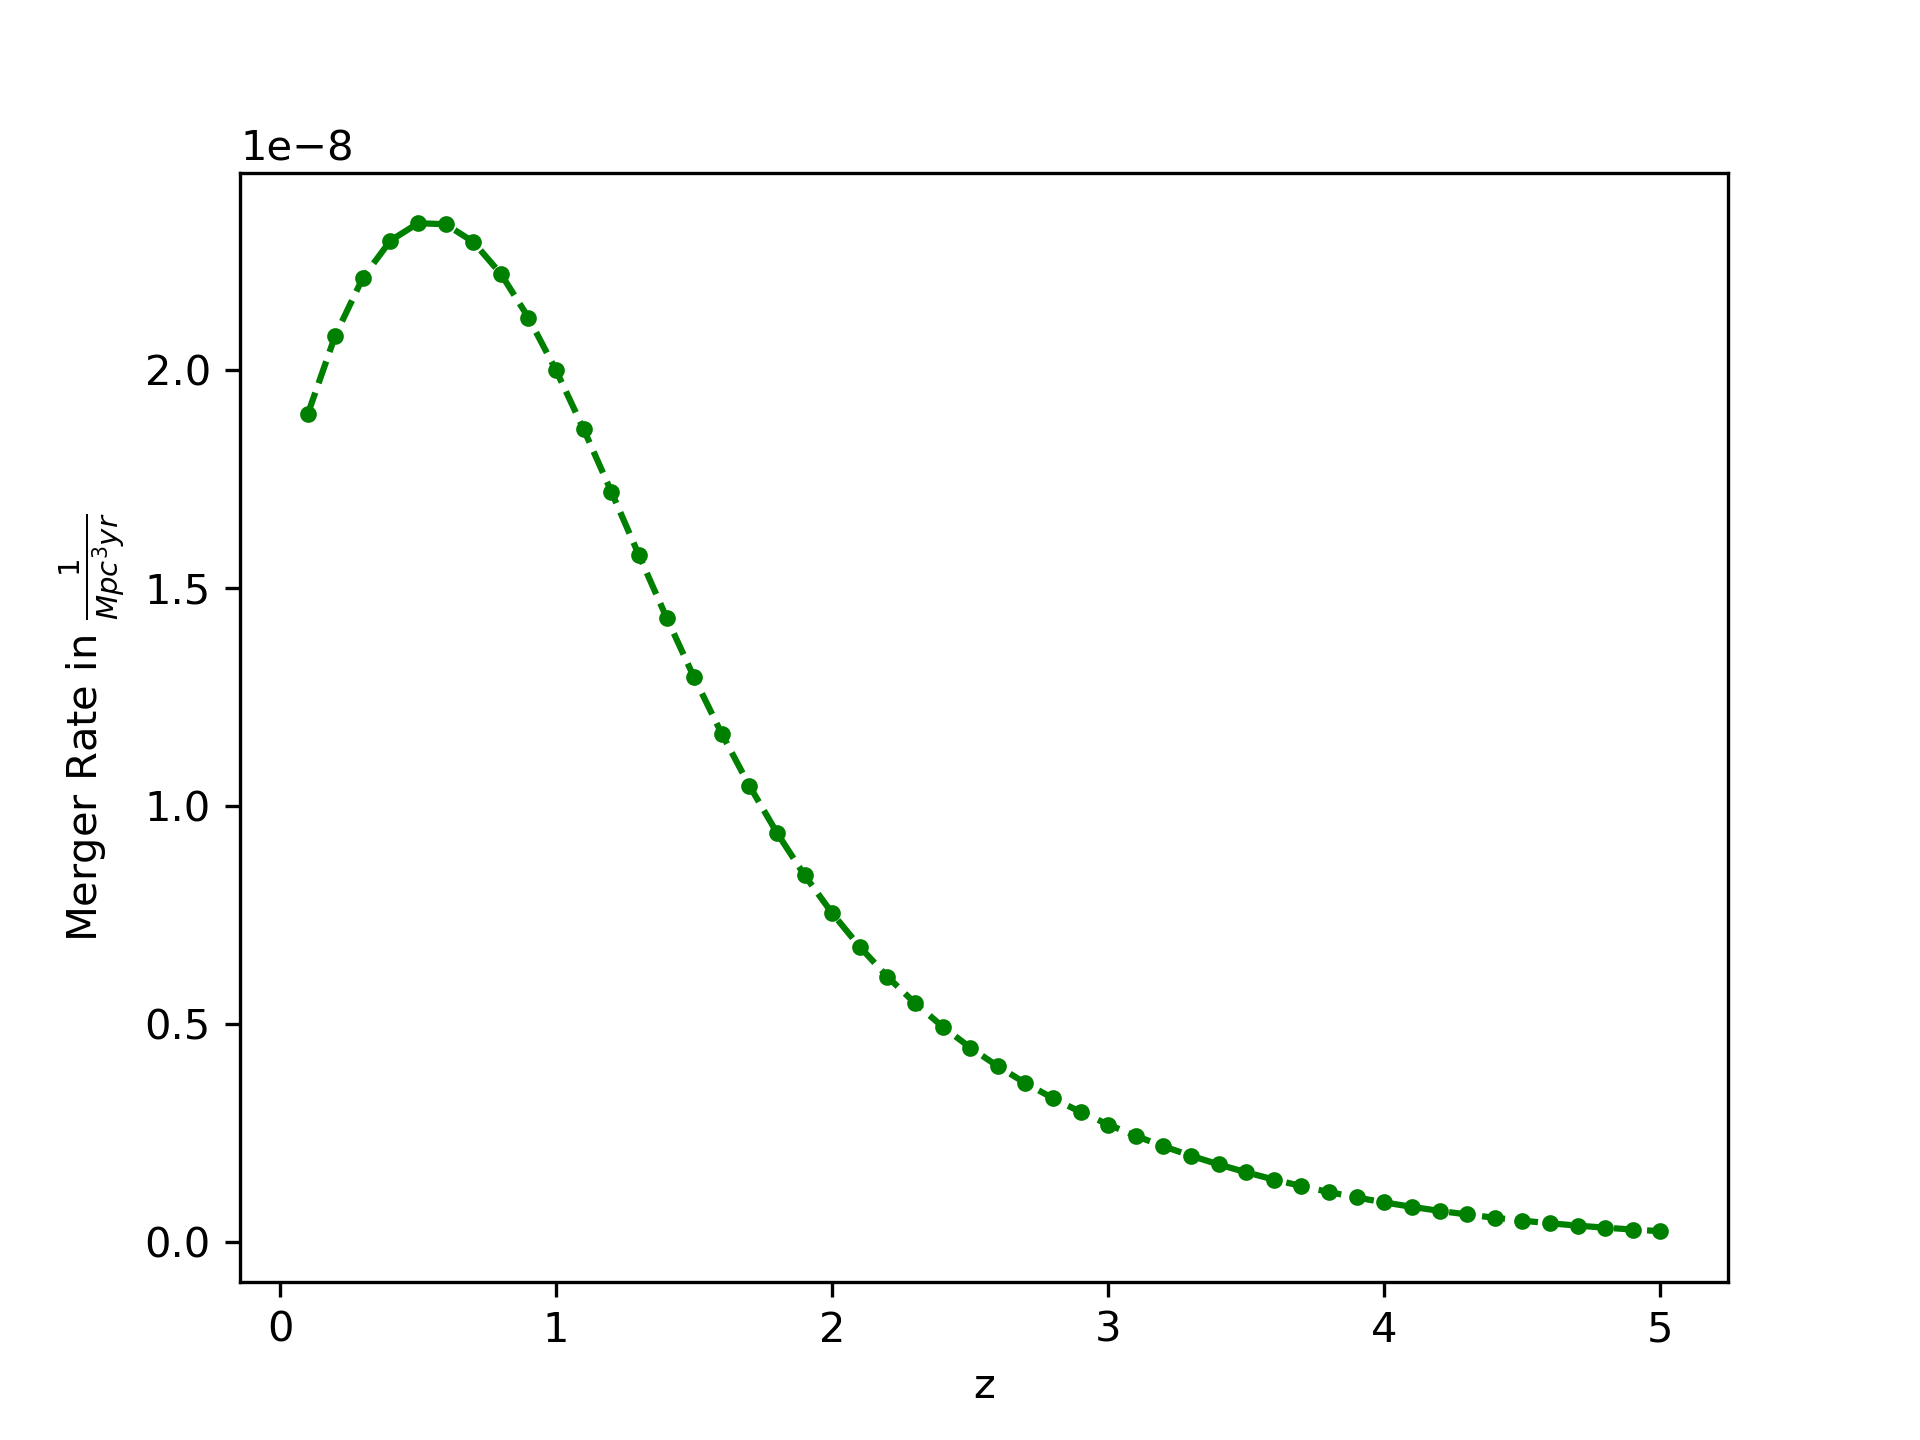
\includegraphics[width=0.9\linewidth]{Images/bbh_merger_rate.png}
    \caption{The BBH merger rate as a function of the redshift z.}
    \label{bbh_merger_rate}
\end{figure} 


\section{Window Function}
\label{window_fct_section}

In Dall'Armi et al. \cite{dallarmi_dipole_2022} we see that the frequency dependence 
of the dipole comes from the evolution bias and the window function. The evolution 
bias accounts for the fact that more sources are created with time. The window 
function is used when we integrate the source functions over the redshift. It weights different redshift regions of the source functions depending on which ones are important for the observable, in this case GW.


\begin{equation}
    \delta_{AGWB}(f_o, \hat{n})=\frac{\Omega_{AGWB}(f_o, \hat{n})-\bar{\Omega}_{AGWB}(f_o)}{\bar{\Omega}_{AGWB}(f_o)}
\end{equation}

\begin{equation}
\label{window_fct_int}
    =\int dz \tilde{W}(f_0, z)\Delta_{AGWB}(f_0, \hat{n}, z)
\end{equation}


In the standard version without frequency dependence, we can already see the influence of the different window functions and redshift ranges.

The different window functions are plotted in Fig.\ref{plot_Cl_window_fct}. The window function determines which part of our source function we count for the density contrast. In the case of a Dirac distribution, we count all parts and skip the integration. This is why that window function leads to a higher angular power spectrum.\\
\begin{figure}[h]
 \centering
 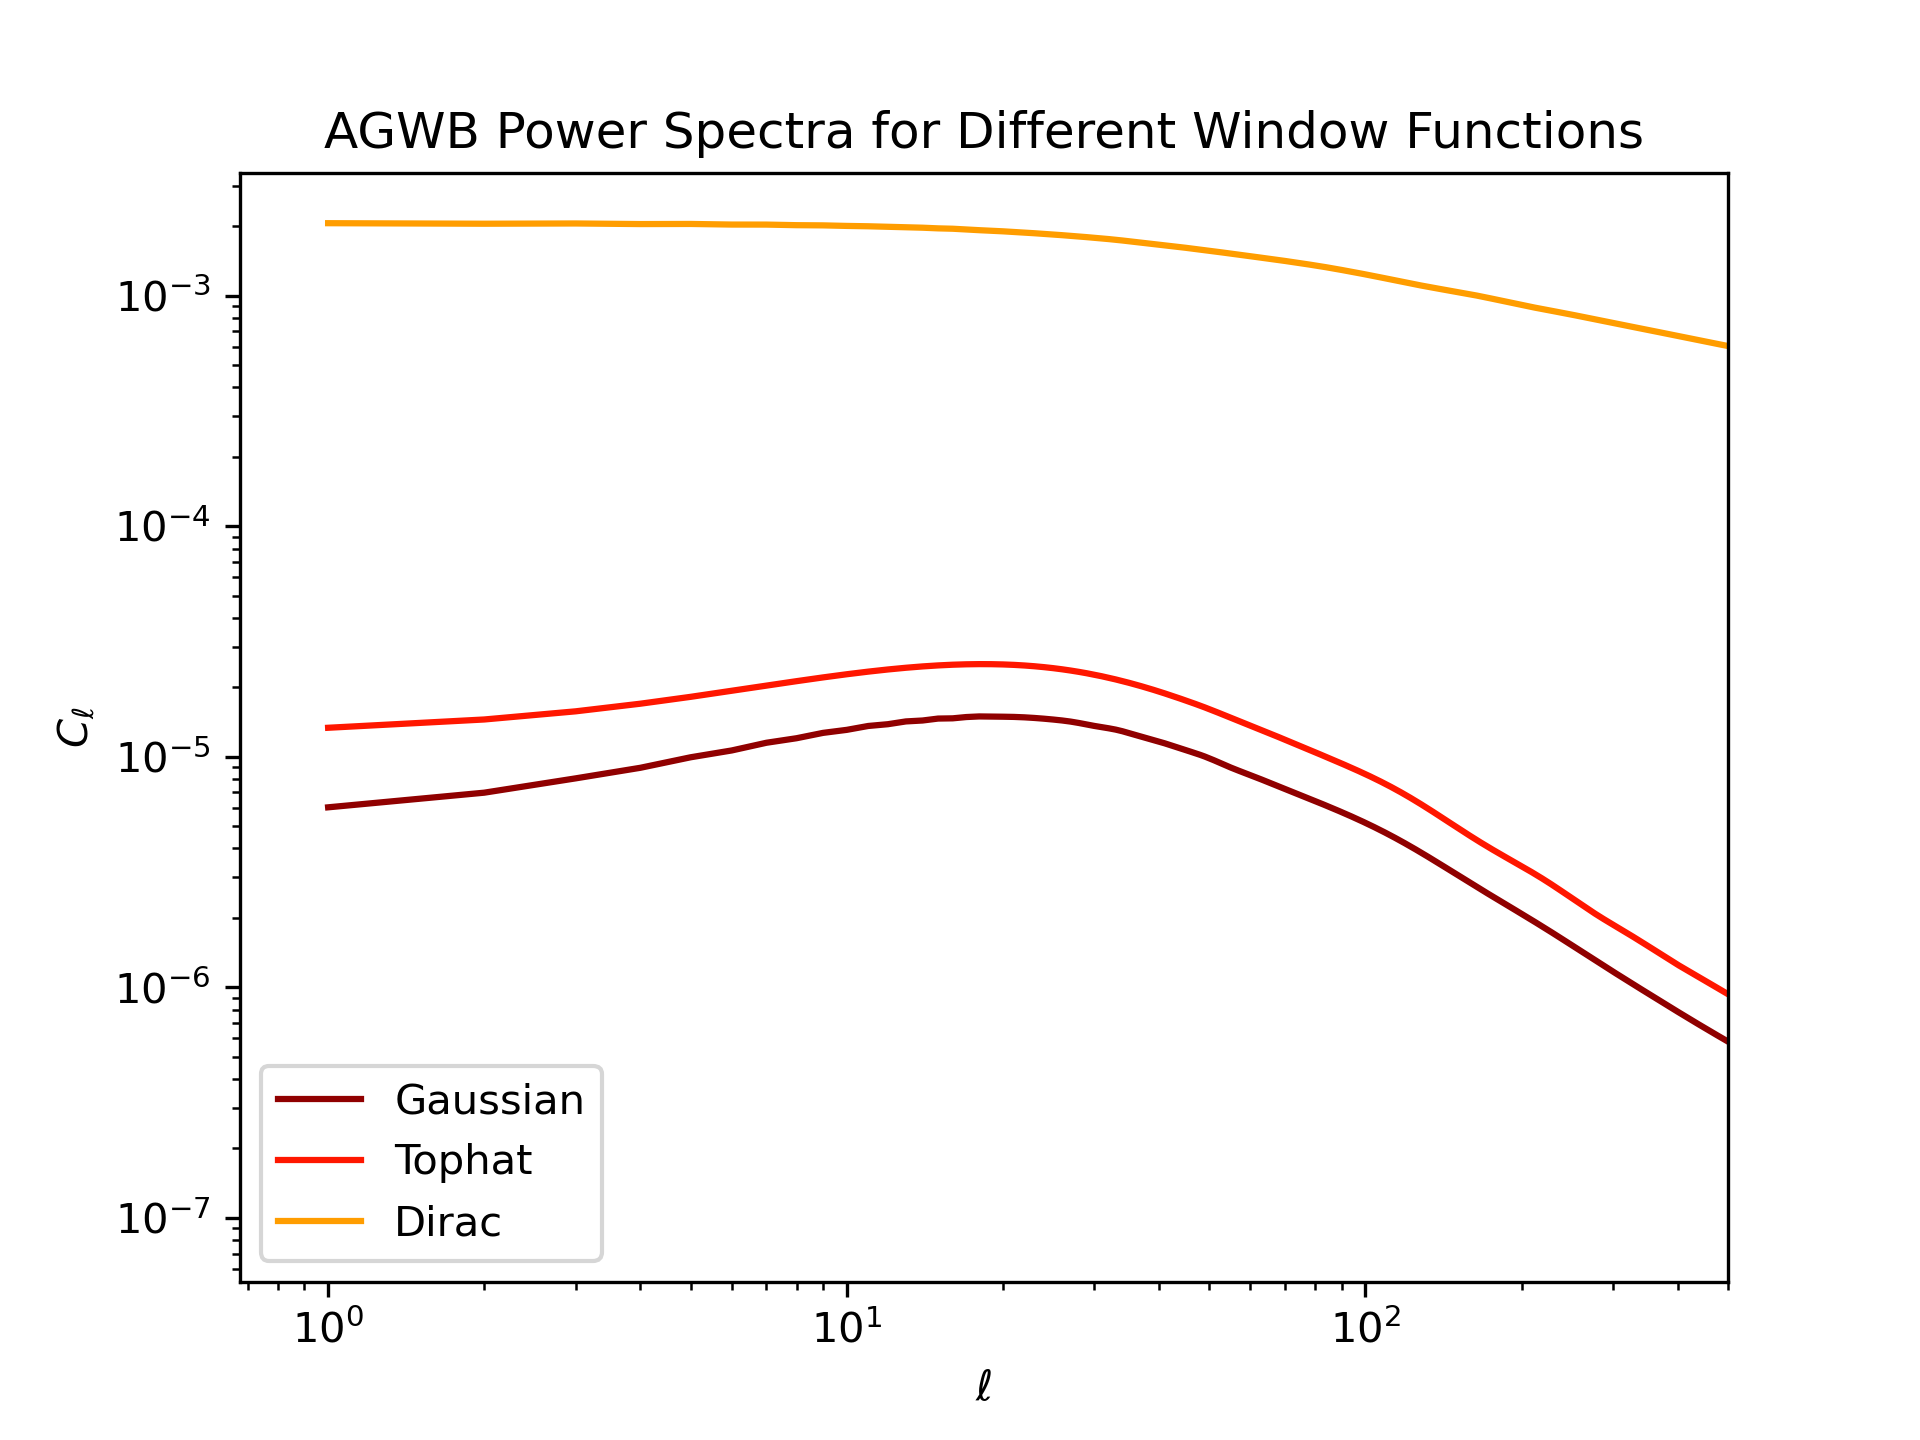
\includegraphics[width=0.7\linewidth]{Images/diff_windows.png}
 \caption{GW angular power spectrum for different window functions.}
 \label{plot_Cl_window_fct}
\end{figure} 

We can see the GW angular power spectrum for different redshifts in Fig.\ref{plot_Cl_redshift}.
The anisotropies are higher for smaller redshifts. This is due to the fact that we have more GW sources at lower redshifts due to structure formation growing linearly with the scale factor $a$.

\begin{figure}[h]
 \centering
 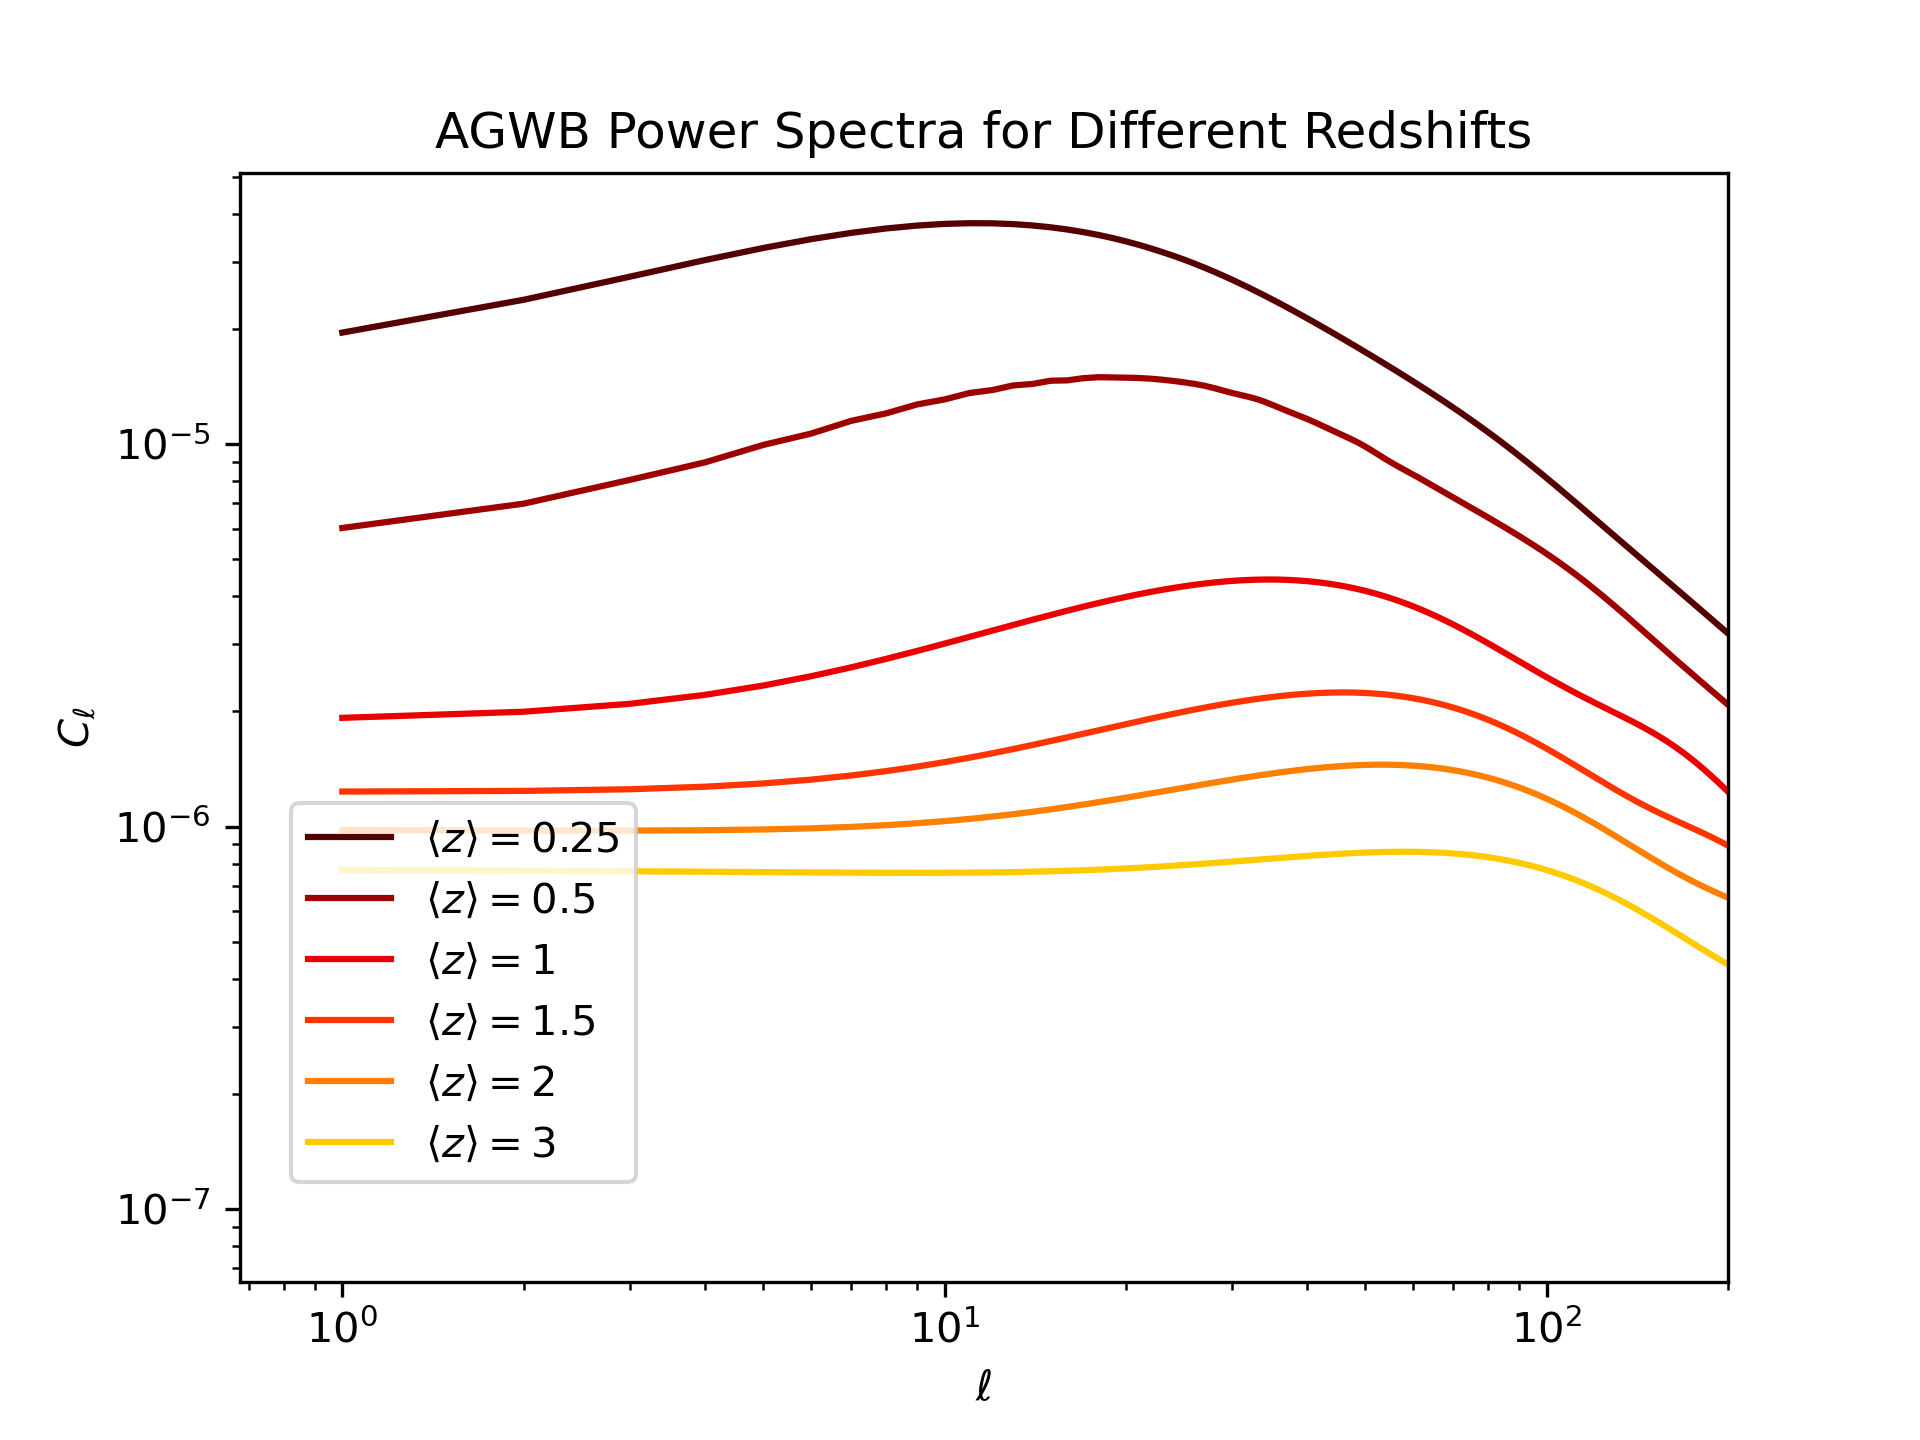
\includegraphics[width=0.7\linewidth]{Images/diff_window_z.png}
 \caption{GW angular power spectrum for different redshifts.}
 \label{plot_Cl_redshift}
\end{figure} 

\begin{equation}
\label{window}
    \tilde{W}(z, f_0)=\frac{f_0}{\rho_c c^2 \bar{\Omega}_{AGWB}(f_0)}
    \frac{R_{BBH}(z)}{(1+z)H(z)} \left. \frac{dE_{GW}}{df_e d\Omega_e}(f_e)\right|_{f_e=(1+z)f_0}
\end{equation}

The window function is normalised using the monopole, which is the same expression integrated over $z$.

\begin{equation}
    \bar{\Omega}_{AGWB}(f_0)= \frac{f_0}{\rho_c}\frac{d\rho_{GW}}{df}
\end{equation}

\begin{equation}
    = \frac{f_0}{\rho_c c^2 } \int \frac{dz}{(1+z)H(z)} R_{BBH}(z) \frac{dE_{GW}}{df_e d\Omega_e}(f_e)
\end{equation}

\begin{figure}
    \centering
    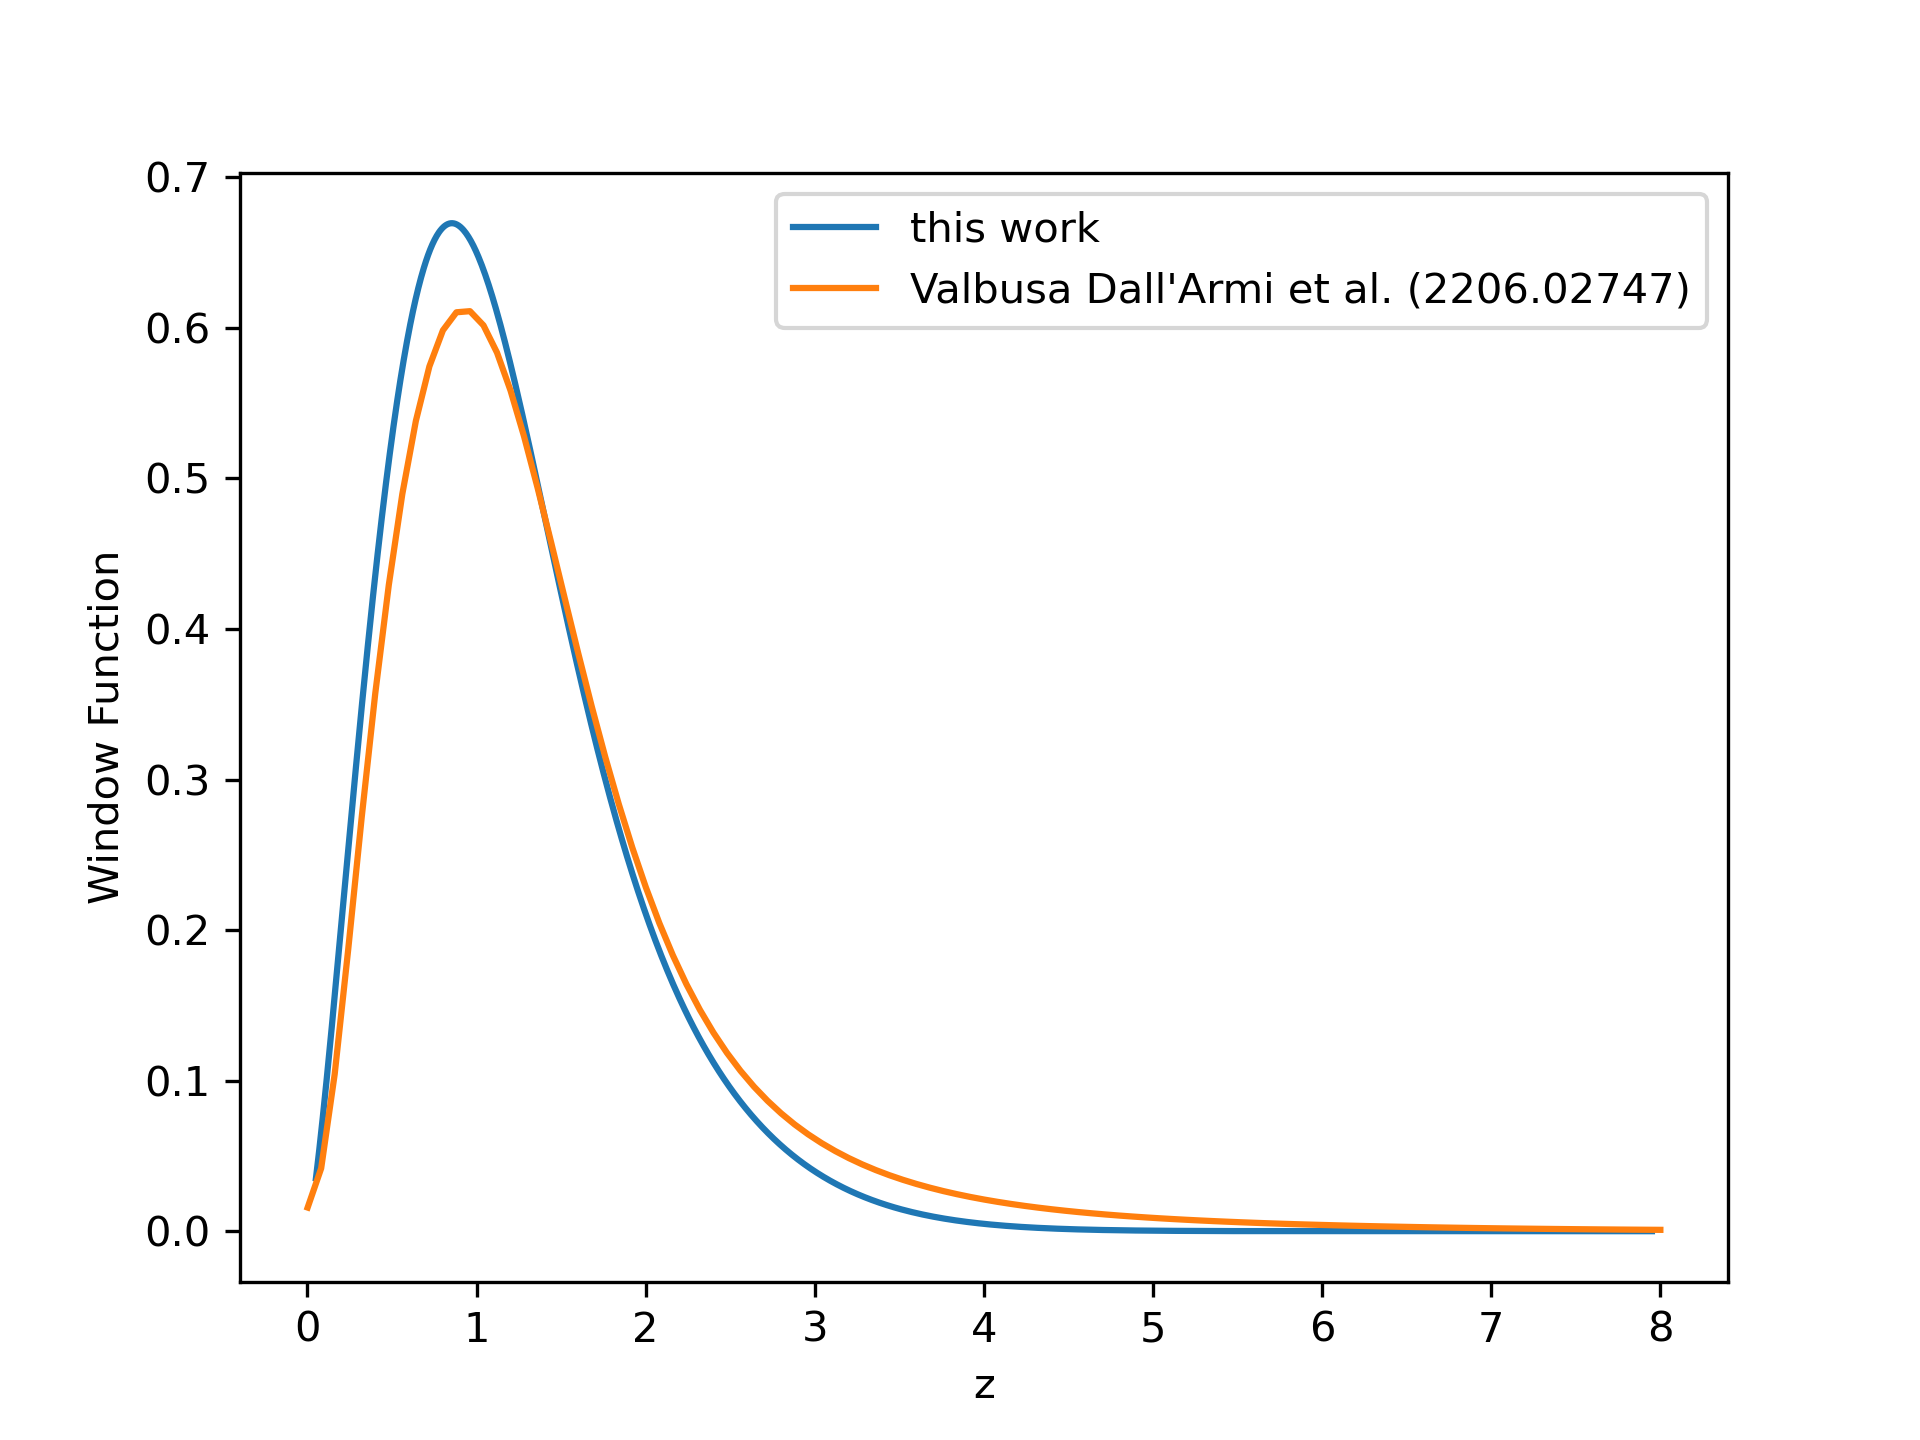
\includegraphics[width=0.8\linewidth]{Images/window_comparison.png}
    \caption[The final window function at 1 Hertz for this code for comparison with \cite{dallarmi_dipole_2022}.]{The final window function at 1 Hertz for this code in blue for comparison with \cite{dallarmi_dipole_2022} in orange.}
    \label{window_comparison}
\end{figure} 
%\vspace{-5cm}
\begin{figure}
    \centering
    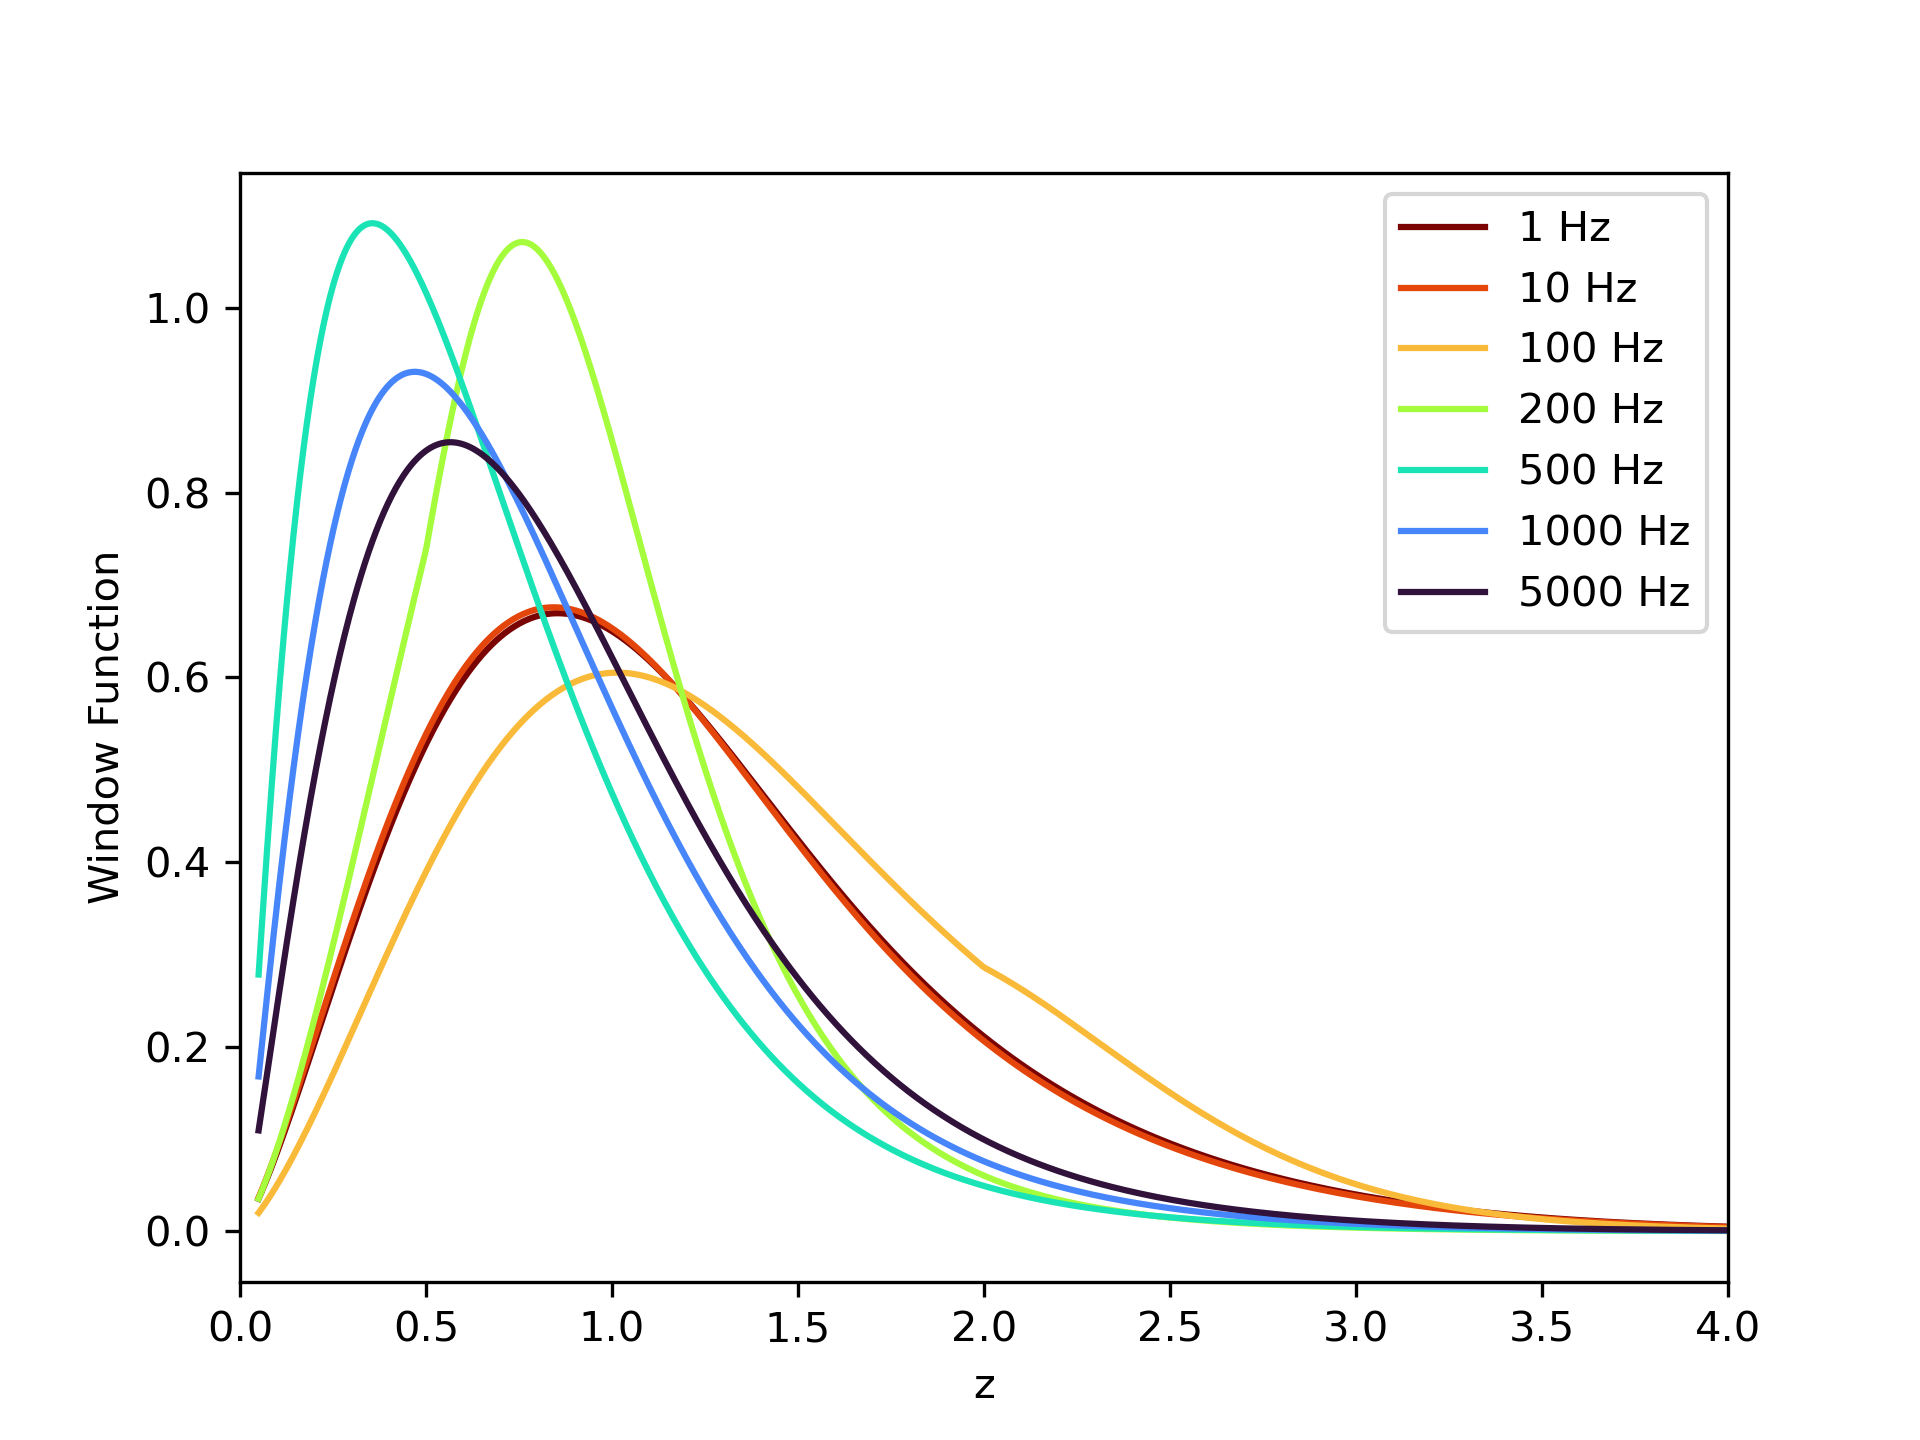
\includegraphics[width=1\linewidth]{Images/window_diff_frequencies.png}
    \caption{The window functions at different observed frequencies.}
    \label{window_frequencies}
\end{figure} 


We then Fourier and Legendre transform the GW density contrast to get Legendre polynomials corresponding to multipoles on the sphere.
\begin{equation}
    \delta_X(f_0, \vec{k}) = \int \frac{d^3\vec{x}}{(2\pi)^\frac{3}{2}} 
    \delta_X(f_0, \vec{x})
\end{equation}
\begin{equation}
    \Delta_l(k, f_0) = \int d\phi \int d\mu \mathcal{P}_l(\mu) 
    \delta(\vec{k}, f_0)
\end{equation}

From that, we can calculate the angular power spectrum using the primordial power 
spectrum.

\begin{equation}
    C_l = 4\pi \int \frac{dk}{k} P(k) \Delta_l \Delta_l^*
\end{equation}

Note, that this $\Delta$ is not the same as in equation \ref{window_fct_def}.


\section{Bias \& Magnification Bias}

If we see GW as a tracer of the underlying dark matter density field, we have to introduce a bias for this tracer, where $\delta$ is again the density contrast.

\begin{equation}
    \delta_{DM}=b_{GW}\delta_{GW}
\end{equation}

\cite{scelfo_gwtimeslss_2018} find this bias to be $1.81$ considering BH from the end-point of stellar evolution (as opposed to primordial BH).

Another bias we consider is the magnification bias. It accounts for gravitational lensing which increases the area of the source and thus decreases the observed number density. Furthermore, fainter object can reach the magnitude threshold due to gravitational lensing.

If one compares the contributions to $\Delta_l^{\rm{AGWB}}$ between {\tt CLASSgal} and the Dall'Armi paper \cite{dallarmi_dipole_2022}, the magnification bias has to be  $s=\frac{2}{5}$ for the expressions to match. To find out why this is the case, I tried some calculations with $\frac{dN}{dz}$, but could not match this value.  After reading the paper by Bertacca et al. \cite{bertacca_projection_2020} (recommended by Lorenzo), one can see that they derive their expressions from 
first principles without introducing the magnification bias separately. 

\section{Evolution Bias}
\label{evo_bias_section}
The evolution bias accounts for the creation of new sources. This is why it depends on the redshift derivative of the merger rate and the energy spectrum of one merger. 
It enters in the projection effects in section \ref{projection_effects}.

\begin{figure}
    \centering
    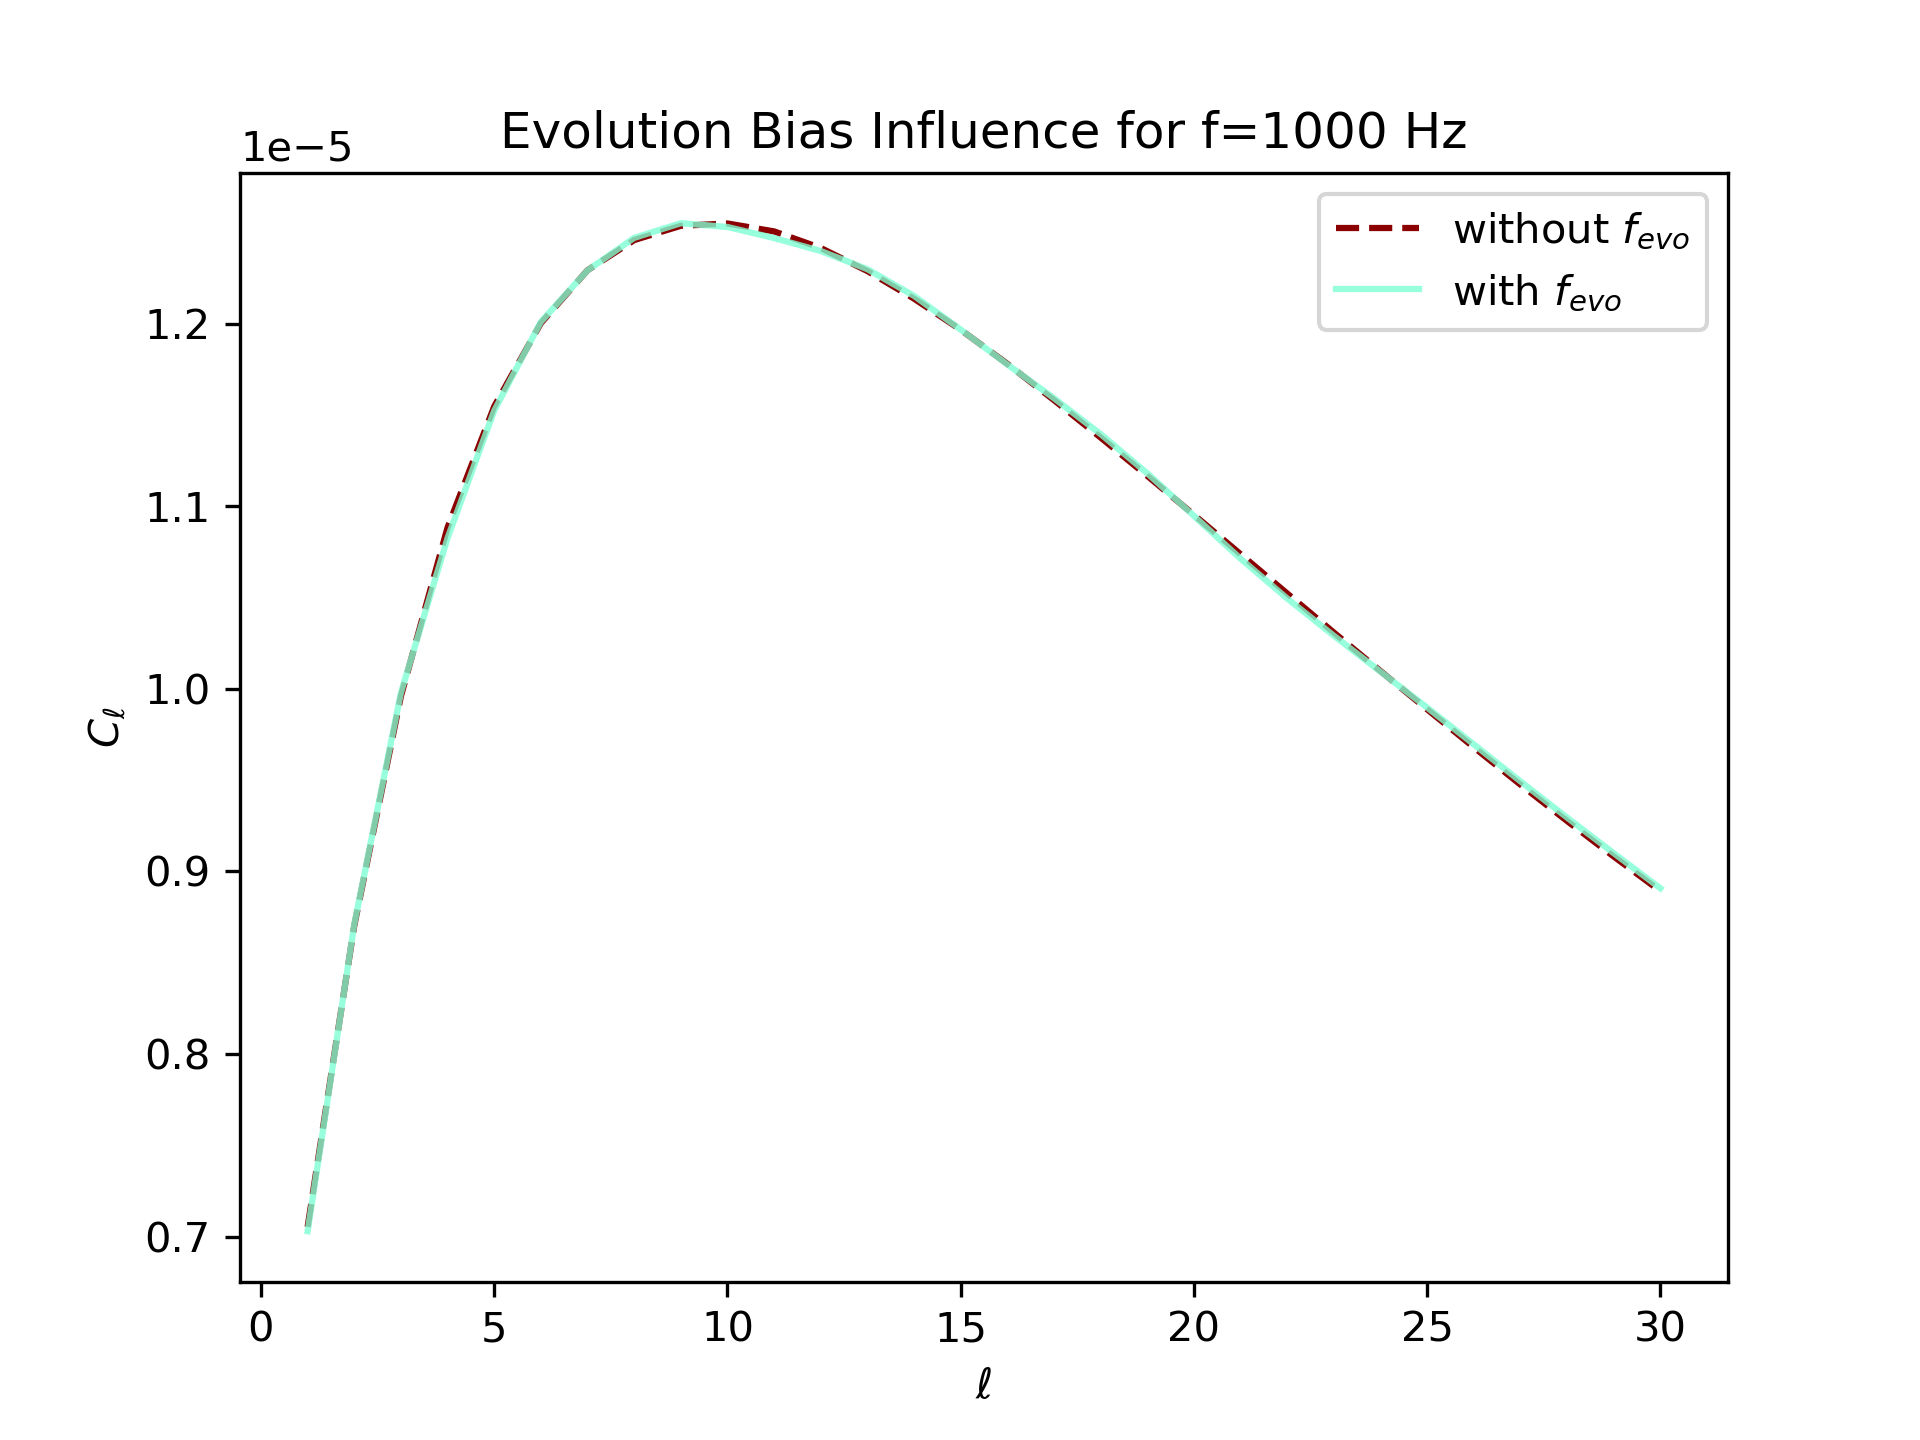
\includegraphics[width=0.8\linewidth]{Images/evo_bias_test.png}
    \caption{The influence of the evolution bias on the angular power spectrum at an observed frequency of 1000 Hertz.}
    \label{evo_bias_plot}
\end{figure} 

We can write this in terms of the derivative of the GW energy flux of the scale factor $a$.
\begin{equation}
    b_e(f_0, z) = \frac{d\ln(F)}{d\ln(a)}(f_0, z)
\end{equation}
\begin{equation}
    = -\frac{1+z}{F(f_0, z)}\frac{dF}{dz}(f_0, z)
\end{equation}
The energy flux of GW is a product of the energy spectrum of one binary, using the waveform by Ajith et al. \cite{ajith_inspiral-merger-ringdown_2011} and the merger rate of binary black holes as a function of redshift.
\begin{equation}
    F(f_0, z) = R_{BBH}(z) \frac{d E_{GW}}{df_e d\Omega_e}(f_0, z)
\end{equation}



In Fig.\ref{evo_bias_plot}, we show the computed angular power spectrum with and without the evolution bias. We can see that it barely influences the overall power spectrum. Computationally, it takes much longer to consider it since the merger rate and energy spectrum are computed again at every step. The merger rate for example contains an integral over the halo mass which increases the runtime.
Because of this minor influence, we neglect the evolution when computing the angular power spectra, but it can easily be activated and deactivated in the {\tt Multi\_CLASS} initialisation file ({\tt disable\_gw\_evo\_bias}).

